\documentclass{amsart}
\usepackage[T1]{fontenc}
\usepackage[utf8]{inputenc}
\usepackage{longtable}
\usepackage{fancyhdr}
\usepackage{amsmath}
\usepackage{amsfonts}
\usepackage{titletoc}
\usepackage{enumitem}
\usepackage{amssymb}
\usepackage[boxed, linesnumbered]{algorithm2e}
\usepackage[left=2cm,right=2cm,top=3cm,bottom=3cm]{geometry}
\usepackage{graphicx}
\usepackage{hyperref}
\usepackage{xcolor}
\usepackage{lastpage} 
\usepackage{setspace}
\usepackage{titlesec}
\usepackage{dsfont}
\usepackage{cleveref}
\usepackage{bm}
\usepackage{extramarks}
\usepackage[colorinlistoftodos,bordercolor=orange,backgroundcolor=orange!20,linecolor=orange,textsize=scriptsize]{todonotes}
\usepackage{subcaption}
\SetAlgoNlRelativeSize{-1}

\geometry{
    top=1in, % Marge supérieure
    bottom=1.5in, % Marge inférieure
    left=1in, % Marge gauche
    right=1in, % Marge droite
    footskip=1in % Espace entre le bas du texte principal et le pied de page
}


\pagestyle{fancy}
\fancyhf{} 

\fancypagestyle{plain}{
    \fancyhf{} 
}
\fancyhead[C]{\normalfont\leftmark}

\titleformat{\section}[hang]
  {\normalfont\Large\bfseries} % Format du texte
  {\thesection{} - } % Préfixe (ex. 1.1 - )
  {1pt} % Espace entre le préfixe et le titre
  {\Large\bfseries} % Format du titre

% Configurer les sous-sections
\titleformat{\subsection}[hang]
  {\normalfont\normalsize\bfseries} % Format du texte
  {\thesubsection{} - } % Préfixe (ex. 1.1.1 - )
  {0pt} % Espace entre le préfixe et le titre
  {\normalsize\bfseries} % Format du titre

% Configurer les sous-sous-sections
\titleformat{\subsubsection}[hang]
  {\normalfont\small\bfseries} % Format du texte
  {\thesubsubsection{} - } % Préfixe (ex. 1.1.1.1 - )
  {0pt} % Espace entre le préfixe et le titre
  {\small\bfseries} % Format du titre
  
\ifdefined\theorem\else \newtheorem{theorem}{Theorem}\fi
\ifdefined\proposition\else \newtheorem{proposition}[theorem]{Proposition}\fi
\ifdefined\definition\else \newtheorem{definition}[theorem]{Definition}\fi
\ifdefined\lemma\else \newtheorem{lemma}[theorem]{Lemma}\fi
\ifdefined\corollary\else \newtheorem{corollary}[theorem]{Corollary}\fi
\ifdefined\remark\else \newtheorem{remark}[theorem]{Remark}\fi
\ifdefined\assumption\else \newtheorem{assumption}{Assumption}\fi
\ifdefined\example\else \newtheorem{example}{Example}\fi
\onehalfspacing


\newcommand{\argmin}{\mathop{\arg\min}}
\crefformat{enumi}{#2#1#3}
\newcommand{\nb}[3]{
		{\colorbox{#2}{\bfseries\sffamily\tiny\textcolor{white}{#1}}}
		{\textcolor{#2}{\text{$\blacktriangleright$}{\textcolor{#2}{#3}}\text{$\blacktriangleleft$}}}}
\newcommand{\rp}[1]{\nb{RP}{red}{#1}}
\newcommand{\af}[1]{\nb{AF}{blue}{#1}}
\newcommand{\bt}[1]{\nb{BT}{orange}{#1}}
\newcommand{\RR}{\mathbb{R}}

\renewcommand{\contentsname}{Table of contents}
\renewcommand{\sectionmark}[1]{\markboth{\thesection. #1}{}}

\begin{document}


\thispagestyle{empty}

\begin{figure}[htbp]
    \centering
    \begin{minipage}[b]{0.22\textwidth}
        \centering
        
\includegraphics[width=\textwidth]{logo/logo.jpg}
    \end{minipage}
    \hfill
    \begin{minipage}[b]{0.25\textwidth}
        \centering
        
\includegraphics[width=\textwidth]{logo/universita di pisa.png}
    \end{minipage}
\end{figure}

\vspace{1.5cm}	

\begin{center}	
    {\huge \bf\ Research Internship  \\
    \vspace{1cm}
    \huge Scenario reduction techniques for two-stage programming. \\
    \vspace{1.5cm}

    \normalsize Field of study : Applied Mathematics \\
    School year : 2023 - 2024 \\



    \vspace{3.3cm}
    \textcolor{red}{Confidentiality notice : }\\
    \color{black}
    \vspace{0.5cm}
    }
\end{center}

\noindent\normalsize \textbf{Author} Romain Pujol  \\
\textbf{Class} 2025 \\

\noindent\textbf{ENSTA Paris supervisor} Sorin-Mihai Grad \\ 
\textbf{Università di Pisa supervisor} Antonio Frangioni \\

\noindent Internship carried out from 13/05/2024 to 02/08/2024. 
\\
Università di Pisa, Lungarno Antonio Pacinotti, 43.


\newpage
\thispagestyle{empty}
\mbox{}
\newpage



%%% PAGE DE CONFIDENTIALITE
%%% PAGE DE CONFIDENTIALITE
%%% PAGE DE CONFIDENTIALITE
%%% PAGE DE CONFIDENTIALITE
%%% PAGE DE CONFIDENTIALITE
%%% PAGE DE CONFIDENTIALITE
%%% PAGE DE CONFIDENTIALITE



\begin{titlepage}

    \vspace*{5cm}
        \Large\textbf{Acknowledgements}
    \vspace{1cm}
    
    \normalsize Thanks.
\end{titlepage}

\newpage

\begin{titlepage}

    \vspace*{1cm}
        \Large\textbf{Abstract} \\
    
    \normalsize Two-stage stochastic optimization problems become very large when the distributions involved have a large number of atoms. The goal is to solve simplified two-stage problems by reducing the size of the initial distribution in order to decrease CPU time. This scenario reduction is ruled by a certain metric, the Wasserstein distance. It is also necessary to ensure that the optimal values obtained from both problems are similar. In order to integrate scenario reduction techniques into the SMS++ ecosystem at the University of Pisa, a special attention is paid to algorithmic efficiency. \\ 
    
    \textbf{Key-words:} Stochastic programming, scenario reduction, Wasserstein distance, greedy algorithm, local-search, stability.
  \\

        \vspace*{1cm}
        \Large\textbf{Résumé} \\
    
    \normalsize Les problèmes d'optimisation stochastique à deux étapes sont de très grande taille lorsque les distributions mises en jeu ont un grand nombre d'atomes. L'objectif sera de résoudre des problèmes à deux étapes simplifiés en \emph{réduisant} la taille de la distribution initiale pour diminuer le temps de calcul. Cette réduction de scénarios est gouvernée par une certaine métrique, la distance de Wasserstein. Il faut aussi être capable de s'assurer que les valeurs optimales obtenues via les deux problèmes sont similaires. Dans le but d'intégrer les techniques de réduction de scénario dans l'écosystème SMS++ de l'Université de Pise, une attention particulière est portée à l'efficacité algorithmique. \\
    
    \textbf{Mots-clés :} Optimisation stochastique, réduction de scénario, distance de Wasserstein, algorithme glouton, recherche locale, stabilité.
    
\end{titlepage}


% Table des matières
\tableofcontents

\newpage
\pagestyle{fancy} % Activer le style fancy
\fancyfoot[R]{\thepage/\pageref{LastPage}} 
\fancyfoot[C]{Romain Pujol / Università di Pisa \\ \textcolor{red}{Confidential / Non confidential report}}
\section{Introduction}
\section{Stability in stochastic programming}\label{stability}
\subsection{Context and notions}
Many Stochastic Programming (SP) models can be written as:
\begin{equation}\label{stochastic}
\min\left\{\int_\Xi F_0\left(x,\xi\right)\text{d}P\left(\xi\right)\:,\: x\in X, \: \int_\Xi F_j\left(x,\xi\right)\text{d}P\left(\xi\right)\leq0, j=1,...,d\right\}.
\end{equation}

Here $X\subset\RR^m$ is closed, $\Xi\subset\RR^s$ is closed, $F_j$ are random lower semi-continuous functions for all $j\in\{0,...,d\}$ and $P$ is a Borel probability measure on $\Xi$. The set $X$ does not depend on $P$ and defines constraints on $x$. The goal of this part is to highlight a specific metric on distributions that would ensure that if two distributions $P$ and $Q$ are close, then the value of both SP models are close. We write:
\begin{align*}
    &\mathcal{X}\left(P\right)=\left\{x\in X, \int_\Xi F_j\left(x,\xi\right)\text{d}P\left(\xi\right)\leq0, j=1,...,d\right\},\\
    &v\left(P\right)=\inf\left\{\int_\Xi F_0\left(x,\xi\right)\text{d}P\left(\xi\right)\:,\: x\in \mathcal{X}\left(P\right)\right\}, \\
    &X^*\left(P\right)=\argmin\left\{\int_\Xi F_0\left(x,\xi\right)\text{d}P\left(\xi\right)\:,\: x\in X, \: \int_\Xi F_j\left(x,\xi\right)\text{d}P\left(\xi\right)\leq0, j=1,...,d\right\}.
\end{align*}
So $\mathcal{X}\left(P\right)$ denotes the feasible set, $v\left(P\right)$ the optimal value of \eqref{stochastic} and $X^*\left(P\right)$ its set of minimizers. For every integer $p\geq 1$, let us define $\mathcal{F}_p\left(\Xi\right)$ a class of measurable functions from $\Xi$ to $\RR$ named locally Lipschitz continuous functions:
\begin{align*}
    &\mathcal{F}_p\left(\Xi\right)=\left\{f:\Xi\to \RR: \lvert f\left(\xi\right)-f\left(\xi'\right)\rvert \leq c_p\left(\xi,\xi'\right)\lVert\xi-\xi'\rVert, \forall \xi,\xi'\in \Xi^2 \right\}, \\
   & c_p\left(\xi,\xi'\right)=\max \left\{1,\lVert\xi \rVert,\lVert\xi'\rVert\right\}^{p-1}.
\end{align*}
When $p=1$, we recall 1-Lipschitz functions. When $p\geq 2$, there exists another dependency on the space $\Xi$ allowing functions with higher and higher variations as $p$ increases. One can note that $F_1\left(\Xi\right)\subset F_2\left(\Xi\right)\subset F_3\left(\Xi\right) \hdots$ For $P,Q\in\mathcal{P}_p\left(\Xi\right)^2$ where $\mathcal{P}_p\left(\Xi\right)=\left\{Q\in\mathcal{P}\left(\Xi\right), \int_\Xi \lVert\xi\rVert^pdQ\left(\xi\right)\right\}$, the latest statement allows us to define $p$-th order Fortet-Mourier metric as:
$$
\zeta_p\left(P,Q\right)=\sup_{f\in\mathcal{F}_p\left(\Xi\right)}\lvert \int_\Xi f\left(\xi\right)\text{d}P\left(\xi\right)-\int_\Xi f\left(\xi\right)\text{d}Q\left(\xi\right)\rvert.
$$
See \href{https://www.imo.universite-paris-saclay.fr/~pierre-loic.meliot/master/exam-2017.pdf}{metric proof}.

\subsection{Result}
Let $Q\in\mathcal{P}\left(\Xi\right)$, we write the perturbed model:
\begin{equation*}
    \min\left\{\int_\Xi F_0\left(x,\xi\right)\text{d}Q\left(\xi\right)\:,\: x\in X, \: \int_\Xi F_j\left(x,\xi\right)\text{d}Q\left(\xi\right)\leq0, j=1,...,d\right\},
\end{equation*}
which is \eqref{stochastic} but with the distribution $Q$ instead of $P$. In this part we will try to compare the notions we have presented in the above part, for instance, we want to bound $\lvert v\left(P\right)-v\left(Q\right)\rvert$ in terms of distribution metrics. \cite[Corollary 14]{romisch_stability_2003} gives:
\begin{theorem}\label{stability_th}
    Let the number of constraints in \eqref{stochastic} be $d=0$ and assume that:
    \begin{enumerate}
        \item The  solution set $X^*\left(P\right)$ is nonempty and $\mathcal{U}$ is an open, bounded neighbourhood of $X^*\left(P\right)$.
        \item The set $X$ is convex and $F_0\left(\cdot,\xi\right)$ is convex on $\RR^m$ for each $\xi\in\Xi$.
        \item there exist constants $L>0, p\geq1$ such that $\frac{1}{L}F_0\left(x,\cdot \right)\in\mathcal{F}_p\left(\Xi\right)$ for each $x\in X\cap cl\mathcal{U}$. 
    \end{enumerate}
    Then there exists a constant $\delta>0$ such that:
    \begin{align*}
        &\lvert v\left(P\right)-v\left(Q\right)\rvert \leq L\zeta_p\left(P,Q\right) \\
        & \emptyset \ne X^*\left(Q\right)\subset X^*\left(P\right)+\Psi_P\left(L\zeta_p\left(P,Q\right)\right)\mathbb{B}
    \end{align*}
    Where $\Psi_p$ is defined in \cite[2.22-2.23]{romisch_stability_2003}. Whenever $Q\in\mathcal{P}\left(\Xi\right)$ with finite $p$-th order absolute moments and $\zeta_p\left(P,Q\right)<\delta$
\end{theorem}
These results has two main points. First, we understand that under a slight perturbation of $P$ (in terms of Fortet-Mourier metric), the optimal value is controlled. The parameter $p$ appears in the third assumption. Second, the set of optimal $x$ of the perturbed model will remain close to the set of optimal $x$ of the original problem. This is a result of stability. 

\subsection{Application to two-stage linear models}\label{two stage}
We consider a linear two-stage model with fixed recourse, this model is generically written as: 
\begin{equation}\label{lp stoch}
    \min_x\left\{c^Tx + \mathbb{E}_\xi\left(\inf_y q\left(\xi\right)^Ty \right)\: :\: Wy\left(\xi\right)=h\left(\xi\right)-T\left(\xi\right)x\:,\: y\left(\xi\right)\geq0\:,\: x\in X \right\}.
\end{equation}
Where $x$ is called the first-stage decision variable, $y$ the second. The general idea of this model is a first-stage decision has to be made before observing $\xi$. The distribution of $\xi$ is known so that $x$ is chosen to ensure the best average outcome. Then after observing $\xi$, the second-stage variable $y$ is determined. One can note that the only decision you make is $x$ as $y$ is determined by $x$ and $\xi$. The term "fixed recourse" highlights the nature of $W$, a fixed matrix that does not depend (in that case) on $\xi$. See \cite{wets_stochastic_1974} for a complete survey on linear two-stage programs with fixed recourse. In order to fit in the definition  \ref{stochastic}, we define:
$$
F_0\left(x,\xi\right)=\begin{cases} 
  c^Tx + \phi\left(q\left(\xi\right), h\left(\xi\right) -T\left(\xi\right)x\right) & h\left(\xi\right)-     T\left(\xi\right)x \in \text{pos}\left(W\right), q\left(\xi\right) \in D, \\
  +\infty & \text{otherwise},
\end{cases}
$$
where $\text{pos}(W)=\left\{Wy, y\in\RR_+^m\right\}$, $D=\left\{u\in\RR^m:\left\{z\in\RR^r:W^Tz \leq u\right\}\ne \emptyset\right\}$ and  \\$\phi\left(u,t\right)=\inf\left\{ u^Ty : Wy=t, y\geq0\right\}$. \ref{lp stoch} can be rewritten as:
\begin{equation}\label{rewrite}
    \min_x\left\{\int_\Xi F_0\left(x,\xi\right)\text{d}P\left(\xi\right): x\in X\right\}. 
\end{equation}
One can note that $d=0$ in this formulation. Let us introduce two assumptions: 
\begin{assumption}\label{h1} For each $\left(x,\xi\right)\in X\times \Xi$ it holds that $h\left(\xi\right)- T\left(\xi\right)x\in \text{pos}\left(W\right), q\left(\xi\right) \in D$.
\end{assumption}
\begin{assumption}
\label{h2} $P\in\mathcal{P}\left(\Xi\right)$ and has a finite $2$-th moment i.e. $\int_\Xi \lVert \xi\rVert^2\text{d}P\left(\xi\right) < \infty$.
\end{assumption}
\noindent Under these two assumptions, equivalence between \ref{lp stoch} and \ref{rewrite} is direct, even though it may look harsh, as both terms inside the integral converge then it is a matter of notation.
%\begin{proof}
    %Let $x\in X$. \Cref{h1} states that $F_0$ will always be written $c^Tx + \phi\left(q\left(\xi\right), h\left(\xi\right) -T\left(\xi\right)x\right)$ when we integrate it on $\Xi$ when $x\in X$.
    %\begin{align*}
    %    \int_\Xi F_0\left(x,\xi\right)\text{d}P\left(\xi\right)&=\int_\Xi c^Tx + \phi\left(q\left(\xi\right), h\left(\xi\right) -T\left(\xi\right)x\right)\text{d}P\left(\xi\right) \\
    %    &= c^Tx + \int_\Xi \inf_y\left\{q\left(\xi\right)^Ty\: :\: Wy=h\left(\xi\right) -T\left(\xi\right)x\right\}\text{d}P\left(\xi\right) \\
    %    &= \left\{c^Tx + \int_\Xi \inf_y\left\{q\left(\xi\right)^Ty\right\}\text{d}P\left(\xi\right)\:,\: Wy=h\left(\xi\right) -T\left(\xi\right)x\right\}
    %\end{align*}
    %There is no problem to split the integral in two as $c^Tx$ is finite, does not depend on $\xi$ and the whole integral is finite aswell. We  used obviously $\int_\Xi\text{d}P\left(\xi\right)=1$. The third equality is a matter of notation. 
%\end{proof}

\begin{proposition}\label{prop 2}
    Let \Cref{h1} be satisfied. Then $F_0$ is a random convex function. Furthermore there exist constants $L>0, \bar{L}>0$, and $K>0$ such that the following holds for all $\xi,\xi'\in\Xi^2$ and $x,x'\in X^2$ with $\max\left\{\lVert x\rVert, \lVert x' \rVert\right\}\leq r$:
    \begin{align}
        \lvert F_0\left(x,\xi\right)- F_0\left(x,\xi'\right)\rvert &\leq Lr\max\left\{1,\lVert \xi\rVert, \lVert \xi'\rVert\right\}\lVert \xi-\xi'\rVert, \label{lips}\\
        \lvert F_0\left(x,\xi\right)- F_0\left(x',\xi\right)\rvert &\leq \bar{L}\max\left\{1,\lVert\xi\rVert^2\right\}\lVert x-x'\rVert, \\
        \lvert F_0\left(x,\xi\right) \rvert&\leq Kr\max\left\{1,\lVert\xi\rVert^2\right\}.
    \end{align}
     
\end{proposition}
\begin{proof}
    See \cite[Proposition 22]{romisch_stability_2003}.
\end{proof}
Thereafter we will work with finite distributions, meaning that $\Xi$ will always be bounded. With $\Xi$ be bounded, we can modify a little what is said in \Cref{lips} from \Cref{prop 2} to our best convenience:
$$
\lvert F_0\left(x,\xi\right)- F_0\left(x,\xi'\right) \leq L'r \lVert \lVert \xi-\xi'\rVert, \text{ with } L'=L\max\left\{1,\max_{\xi\in\Xi}\lVert\xi\rVert\right\}.
$$
This means that there exists a constant $C>0$ such that $\frac{1}{C}F_0\left(x,\cdot\right)\in\mathcal{F}_1\left(\Xi\right)$ for each $x\in X$ hence if we fix $U$ an open, bounded neighbourhood of $X^*\left(P\right)$ the result hold for each $x\in X\cap \text{cl}U\subset X$. In other words, condition (3) of \Cref{stability_th} is verified with $p=1$.

\begin{corollary}
    Let both assumptions \Cref{h1} and \Cref{h2} be satisfied, $\Xi$ be bounded and let $X^*\left(P\right)$ be nonempty and $\mathcal{U}$ be an open, bounded neighbourhood of $X^*\left(P\right).$ Then there exist constants $L>0$ and $\delta >0$ such that:
    \begin{align*}
        \lvert v\left(P\right)-v\left(Q\right)\rvert \leq L\zeta_1\left(P,Q\right) \\
        \emptyset \ne X^*\left(Q\right)\subset X^*\left(P\right)+\Psi_P\left(L\zeta_1\left(P,Q\right)\right)\mathbb{B}
    \end{align*}
    whenever $Q\in\mathcal{P}\left(\Xi\right)$ and has a finite $1$-th moment and $\zeta_1\left(P,Q\right)<\delta$.
\end{corollary}
\begin{proof}
    This is an application of \Cref{stability_th} with $p=1$ where both assumptions are sufficient to ensure that conditions (2), (3) of \Cref{stability_th} are verified. Condition (1) is verified when the problem is well posed, meaning that there exists a solution. See \cite[Proposition 22]{romisch_stability_2003}.
\end{proof}
\begin{remark}
    In \cite{romisch_stability_2003}, they do not assume that $\Xi$ is bounded and then the results hold with $p=2$.
\end{remark}
Consider now a two-stage model with a distribution $P=\sum_{i\in I}\delta_{x_i}p_i$ with $n$ atoms, $n$ is large. We may want to find another distribution $Q$ with a reduced number of atoms close to $P$ in terms of $\zeta_1$ so that $\lvert v\left(P\right)-v\left(Q\right)\rvert$ is controlled. Finding such a distribution $Q$ would reduce run time when solving the associated SP on a computer. Let us recall the definition of the $p$-th order Fortet-Mourier metric:
$$
\zeta_1\left(P,Q\right)=\sup_{F\in\mathcal{F}_1\left(\Xi\right)}\lvert \int_\Xi F\left(\xi\right)\text{d}P\left(\xi\right)-\int_\Xi F\left(\xi\right)\text{d}Q\left(\xi\right)\rvert,
$$
where $\mathcal{F}_1\left(\Xi\right)=\left\{F:\Xi\to \RR: \lvert F\left(\xi\right)-F\left(\tilde{\xi}\right)\rvert \leq \lVert\xi-\xi'\rVert, \forall \xi,\xi'\in \Xi^2 \right\}$. Computing this upper bound on the Lipschitz functions tends to be hard nay impossible. We introduce $U\left(P,Q\right)$ the set of joint distributions whose marginals are $P$ and $Q$ and the type-$\ell$ Wasserstein distance: $$
W_\ell\left(P,Q\right) = \left\{\min_{\pi\in U\left(P,Q\right)}\int_{\Xi^2}\lVert \xi-\xi'\rVert^l \text{d}\pi\left(\xi,\xi'\right)\right\}^{1/l}.$$
Where $\lVert \cdot \rVert$ denotes the norm on $\Xi$ used to define $\mathcal{F}_1\left(\Xi\right)$. The next idea is to bound $\zeta_1$ by any $W_\ell$ which would be easier to compute.
\begin{align*}
    \zeta_1\left(P,Q\right)&= \sup_{F\in\mathcal{F}_1\left(\Xi\right)}\lvert \int_\Xi F\left(\xi\right)\text{d}P\left(\xi\right)-\int_\Xi F\left(\xi\right)\text{d}Q\left(\xi\right)\rvert, \\
    &=\mathcal{W}_1\left(P,Q\right), \quad \mathcal{W} \text{ being the dual of } W \text{, see \cite{peyre_computational_2019}[Chapter 6],}\\
    &= W_1\left(P,Q\right), \quad \text{due to the duality theorem of Kantorovich-Rubinstein.}
\end{align*}
In order to choose a $\ell$ that will simplify the work, $\ell\in\left\{1,2\right\}$ actually, we will prove that $W_1\left(P,Q\right)\leq W_\ell\left(P,Q\right)$ for any $\ell \geq 1$.  Let $\ell >1$, $q>1$ such that $\frac{1}{\ell}+\frac{1}{q}=1$ and $\pi\in U\left(P,Q\right)$:
\begin{align*}
W_1\left(P,Q\right)&\leq \int_{\Xi^2}\lVert \xi-\xi'\rVert \text{d}\pi\left(\xi\times\xi'\right),\: \pi \text{ may not be optimal,} \\ &\leq \left(\int_{\Xi^2} \lvert 1\rvert^{q}\text{d}\pi\left(\xi\times\xi'\right)\right)^{1/q} \left(\int_{\Xi^2}\lVert \xi-\xi'\rVert^\ell\text{d}\pi\left(\xi\times\xi'\right)\right)^{1/\ell}, \: \text{due to Hölder's inequality} \\
&=\left(\int_{\Xi^2}\lVert \xi-\xi'\rVert^\ell\text{d}\pi\left(\xi\times\xi'\right)\right)^{1/\ell}.
\end{align*}
We can now take the infimum over $\pi$ what gives:
$$
W_1\left(P,Q\right)\leq W_\ell\left(P,Q\right).
$$
For a two-stage linear model, we have finally proven that for $\ell\geq1$, there exists a constant $L>0$ such that:
$$
\lvert v\left(P\right)-v\left(Q\right)\rvert \leq LW_\ell\left(P,Q\right).
$$
Thereafter we will consider a finite distribution $P$ and attempt to find another distribution $Q$ with fewer atoms with the idea of minimizing the type-$\ell$ Wasserstein distance between them. This would control the term: $\lvert v\left(P\right)-v\left(Q\right)\rvert$. We will work with $\ell\in\left\{1,2\right\}$ for the theoretical part and $\ell=2$ for every simulation.

\section{Wasserstein distance with finite distribution}

In this part, we present tools and concepts useful for scenario reduction aswell as their guarantees and limits. Results derive from \cite{rujeerapaiboon_scenario_2022}. 

\subsection{Introduction to Wasserstein distance}
In the case of discrete distributions $P=\sum_{i\in I}p_i\delta_{x_i}$ and $Q=\sum_{j\in J}q_j\delta_{y_j}$. The type-$l$ Wasserstein distance between $P$ and $Q$ is defined as :  
\begin{definition}{Type-$\ell$ Wasserstein distance}
$$
d_\ell(P,Q)=\left(\min_{\pi\in\mathbb{R}_+^{\lvert I\rvert\times\lvert J\rvert}}\left\{ 
\sum_{i\in I}\sum_{j\in J}\pi_{ij}\lVert x_i-y_j\rVert^l \: \text{ : } \:  \begin{aligned}
& \sum_{j\in J}\pi_{ij}=p_i \: \forall i\in I \\
& \sum_{i\in I}\pi_{ij}=q_j \: \forall j\in J
\end{aligned}\right\}\right)^{1/\ell}.
$$
\end{definition}

\begin{remark}
    A more general definition can be written by replacing the norm with a particular distance between objects $x_i$ and $y_j$. 
\end{remark}
For $l\geq1$, this mathematical expression meets the requirements of a distance. Values are positive, symmetry is direct, definiteness requires more work but the idea is to start by proving that $d_\ell\left(P,Q\right)=0$ implies that $\text{supp}\left(P\right)=\text{supp}\left(Q\right)$, concluding will be easy after that. Triangle inequality derives from the gluing lemma, see e.g. \cite[Chapter 1]{peyre_computational_2019}. For $l\in\mathopen{]}0,1\mathclose{]}, d_\ell^\ell$ is a distance. A pro of this particular distance is to rely on the underlying structure meaning the norm. The philosophy of this distance is to measure the minimum cost of moving weights from $x_i$ to $y_j$ where costs are defined by the norm.
\newline

Let $\mathcal{P}_U(X,n)$ denote the set of all \emph{uniform} discrete distribution on $X\subset R^d$ with $n$ distinct scenarios (do not mind if I use scenarios instead of scenari) and $\mathcal{P}(X,m)$ denote the set of discrete distributions on $X\subset R^d$ with \emph{at most} m scenarios. 
\newline

As presented in the conclusion of \ref{stability}, we want to find a distribution that minimizes the Wasserstein distance over a particular set of distribution. Two types of reduction are typically presented. The continous scenario reduction problem :
$$
C_\ell(P,m)=\min_Q\left\{d_\ell(P,Q),\: Q\in\mathcal{P}(\mathbb{R}^d,m)\right\}, 
$$
and the discrete scenario reduction problem :
$$
D_\ell(P,m)=\min_Q\left\{d_\ell(P,Q),\: Q\in\mathcal{P}(\text{supp}(P),m)\right\}.
$$

Let $P$ be a finite distribution on $\RR^d$. Obviously $\text{supp}(P)\subset \RR^d$ what leads to $C_\ell(P,m)\leq D_\ell(P,m)$. Discrete scenario reduction may be sometimes more suitable as continous scenario reduction can generate atoms that may be nonsensical in a particular context.

\subsection{Results of scenario reduction}
In this part, we provide bounds on the Wasserstein distance between an original distribution of $n$ atoms and its reduced one with $m<n$ atoms. Let $X\subset \RR^d$ and $\lVert \cdot \rVert$ be a norm on $X$. We restrict ourselves to distribution whose atoms lie within the unit ball and $\frac{1}{n}\sum_ix_i=0$. This is a legal assumption because of first repositionning a distribution does not affect $C_\ell$, second the positive homogeneity of $C_\ell$. Let $P=\sum_{i\in I}p_i\delta_{x_i}$, $\text{card}\left(I\right)=n<+\infty$, $1<m<n$, $\lambda\in\RR_+^*$ and $a\in\RR^d$:
$$
C_\ell\left(P,m\right)=\frac{1}{\lambda} C_\ell\left(\sum_{i\in I}p_i\delta_{\lambda x_i+a},m\right).
$$
We will work with uniform distribution $P\in\mathcal{P}_U\left(\RR^d,n\right)$ with the idea that the distributions derive from sampling and if not you can multiply atoms around a point of high probability. A goal of this part is to quantify and study the worst case of scenario reduction defined by:
$$    \bar{C}_\ell\left(n,m \right)=\left\{\max_{P\in\mathcal{P}_U(\mathbb{R}^d,n)}C_\ell(P,m)\: :\: \text{supp}(P)\in B(0,1)\right\}.
$$
Let us write a first bound that we will tighten thereafter, let $P\in\mathcal{P}_U(\mathbb{R}^d,n)$:
$$C_\ell\left(P,m\right)\leq C_\ell\left(P,1\right)\leq d_\ell\left(P,\delta_{0_{\RR^d}}\right)\leq 1.$$
As the right-hand side of the equation does not depend on $P$, one can take the upper bound over $P\in\mathcal{P}_U\left(\RR^d,n\right)$ and write that:
$$
\bar{C}_\ell\left(n,m \right)\leq1.
$$
Let $\mathfrak{P}(I,m)$ be the family of m-set partitions of $I$. Following \cite{rujeerapaiboon_scenario_2022}, we write $\{I_j\}$ an element of $\mathfrak{P}(I,m)$ and $I_j$ for $j\in\{1,..,m\}$ a set of the partition $\{I_j\}$.
\begin{theorem}{Reformulation}\label{theorem1}
$$C_\ell(P,m)=\min_{\{I_j\}\in \mathfrak{P}(I,m)}\left\{ \frac{1}{n}\sum_{j\in J}\min_{y_j\in\mathbb{R}^d}\sum_{i\in I_j}\lVert x_i-y_j\rVert^\ell \right\}^{1/\ell}.$$
\end{theorem}
\begin{remark}
    This reformulation takes the most of \Cref{closed formula}.
\end{remark}
Assume that we use the euclidean norm. In the case $\ell=1$, $y_j^*$ is attained by any geometric median. Now if $\ell=2$, the inner minimum can be found easily, gradient of the inner function is well-defined and minimizing with  no constraints gives: $$y_j^*=\text{mean}\left(I_j\right)=\frac{1}{\lvert I_j\rvert}{\sum_{i\in I_j}x_i}.$$ 
\begin{theorem}{Tighter bounds}
    $$\sqrt{\frac{n-m}{n-1}}\leq\bar{C_1}\left(n,m\right)\leq\bar{C_2}\left(n,m\right)\leq\sqrt{\frac{n-m}{n-1}}.$$
\end{theorem}
\subsection{Discrete scenario reduction}
Reduced distributions obtained via continuous scenario reduction are always at least as good as reduced sets obtained via discrete scenario reduction. We will try to quantify the gap between the solution of both problems. More precisely, in this part we find for $\ell\in\{1,2\}$: 
$$\underline{\kappa_\ell}\left(n,m\right)\cdot C_\ell\left(P,m\right)\leq D_\ell\left(P,m\right)\leq \bar{\kappa_\ell}\left(n,m\right)\cdot C_\ell\left(P,m\right).$$
The goal is to find the largest $\underline{\kappa_\ell}\left(n,m\right)$ and smallest $\bar{\kappa_\ell}\left(n,m\right)$ so the bounds are as tight as possible. Solving the continuous problem will give bounds on the discrete. It's easy to argue that : 
$$
\underline{\kappa_\ell}\left(n,m\right)\geq1.
$$
Because we have already proven: 
$$
C_\ell\left(P,m\right)\leq D_\ell\left(P,m\right).
$$
Similarly to what we have done just before, it is time to reformulate the discrete scenario reduction problem such as:
\begin{theorem}\label{reformulation 2}
    For any type-l Wasserstein distance induced by any norm $\lVert\cdot\rVert$, the discrete scenario reduction problem admits the following reformulation: 
    $$
    D_\ell\left(P,m\right)=\min_{\{I_j\}\in\mathfrak{P}\left(I,m\right)}\left[ \frac{1}{n}\sum_{j\in J}\min_{y_j\in\{x_i : i\in I_j\}}\sum_{i\in I_j}\lVert x_i-y_j\rVert^\ell\right]^{1/\ell}.
    $$
\end{theorem}

What follows assumes that $n\geq2, m\in\{1,...,n-1\}$ and $d\geq2.$
\paragraph{\textbf{Type-2 Wasserstein distance.}}
\begin{theorem}
    The upper bound $\bar\kappa_2\left(n,m\right)$ satisfies $\bar\kappa_2\left(n,m\right)\leq \sqrt{2}$ for all n, m.
\end{theorem}
\begin{proof} 
    The proof is very interesting for one's intuition. \textbf{In the first step}, we prove the result for $m=1$. Let $P=\frac{1}{n}\sum_{i\in I}\delta_{x_i}\in\mathcal{P}_U\left(\RR^d,n\right)$. W.l.o.g., we can assume that $\frac{1}{n}\sum_{i\in I}x_i=0$ and $\frac{1}{n}\sum_{i\in I}\lVert x_i\rVert^2=1$ because re-positionning does not affect $C_\ell$ and $D_\ell$ and re-scaling affects equally $D_\ell$ and $C_\ell$ (\rp{refaire un appendice propre sur cela}).
    \newline
    The first reformulation of \Cref{theorem1} gives that :
    $$
    C_2\left(P,1\right)=\left[\frac{1}{n}\sum_{i\in I}\lVert x_i-\text{mean}(I)\rVert_2^2\right]^{1/2}=1.
    $$
    Now we use the reformulation of \Cref{reformulation 2} in order to write:
    $$
    D_2\left(P,1\right)=\left[\frac{1}{n}\min_{j\in I}\sum_{i\in I}\lVert x_i-x_j\rVert^2_2\right]^{1/2}.
    $$
    The $\left(j, x_j\right)$ minimizing this expression minimizes the sum of squared distances with all atoms of $P$. Let us develop:
    \begin{align*}
    D_2\left(P,1\right)&=\left[\frac{1}{n}\min_{j\in I}\sum_{i\in I}\left(\rVert x_i\rVert^2_2-2x_i^Tx_j+\rVert x_j\rVert^2_2\right)\right]^{1/2}\\&=\left[\frac{1}{n}\sum_{i\in I}\lVert x_i\rVert_2^2-\frac{2}{n}\min_{j\in I}\left(\sum_{i\in I}x_i^T\right)x_j+\min_{j\in I}\lVert x_j\rVert^2_2\right]^{1/2} \\&=\left(1+\min_{j\in I}\lVert x_j\rVert^2_2\right)^{1/2}\leq\sqrt{2}.
    \end{align*}
Where we have used $\text{mean}(I)=0$ to write the third equality. The final inequality is due to: $$\min_{j\in I}\lVert x_j\rVert^2_2=\frac{1}{n}\sum_{i\in I}\min_{j\in I}\lVert x_j\rVert^2_2\leq \frac{1}{n}\sum_{i\in I}\lVert x_j\rVert^2_2=1$$. Then: $$D_2\left(P,1\right)\leq\sqrt{2}$$
In order to make it complete for the case $m=1$. Let $P=\frac{1}{n}\sum_{i\in I}\delta_{x_i}\in\mathcal{P}_U\left(\RR^d,n\right)$. We consider $P'=\frac{1}{n}\sum_{i\in I}\delta_{\frac{x_i-\text{mean}(I)}{r}}$ with $r=\sqrt{\sum_{i\in I}\rVert x_i-\text{mean}(I)\lVert^2_2}$. $P'$ verifies the aforementionned conditions. Then we have: 
$$
\frac{D_2\left(P,1\right)}{C_2\left(P,1\right)}=\frac{rD_2\left(P',1\right)}{rC_2\left(P',1\right)}=\frac{D_2\left(P',1\right)}{C_2\left(P',1\right)}\leq \sqrt{2}.
$$
Finally, we have : $$\bar\kappa_2\left(n,1\right)\leq\sqrt{2}.$$
\newline

\textbf{Step 2} extends the result for $n,m\in\{1,...,n-1\}$ using the result above for $m=1$ by decomposing with $m$ scenario reduction problem with 1 atom. Let $P\in\mathcal{P}_U\left(\RR^d,n\right). $ With \Cref{theorem1}, we can write that :
$$
C_2\left(P,m\right)=\min_{\{I_j\}\in \mathfrak{P}(I,m)}\left\{ \frac{1}{n}\sum_{j\in J}\sum_{i\in I_j}\lVert x_i-\text{mean}\left(I_j\right)\rVert^2_2 \right\}^{1/2}
$$
For an optimal $\{I_j^*\}\in\mathfrak{P}\left(I,m\right)$, we have that :
$$
C_2\left(P,m\right)=\left(\frac{1}{n}\sum_{j\in J}\sum_{i\in I_j^*} \lVert x_i-\text{mean}\left(I_j^*\right)\rVert^2_2\right)^{1/2}=\left(\frac{1}{n}\sum_{j\in J}\lvert I_j^*\rvert C^2_{2,j}\right)^{1/2}.
$$
with $C_{2,j}=\left(\frac{1}{\lvert I_j^*\rvert}\sum_{i\in I_j^*}\lVert x_i -\text{mean}\left(I_j\right)\rVert^2_2\right)$. So typically,  $C_{2,j}=C_2\left(\frac{1}{\lvert I_j^*\rvert}\sum_{i\in I_j^*}\delta_{x_i},1\right)$ as reminded for \textbf{step 1}.

With $D_{2,k}=\min_{i\in I_k}\left(\frac{1}{\lvert I_k\rvert}\sum_{j\in I_k}\lVert x_j -x_i\rVert^2_2\right)^{1/2}$ and \Cref{reformulation 2}, we have the analogous expression for an optimal $\{I_k^*\}\in\mathfrak{P}\left(I,m\right)$ : 
$$
D_2\left(P,m\right)=\left[ \sum_{k\in K}\frac{\lvert I_k^*\rvert}{n}D_{2,k}^2\right]^{1/2}\leq \left[ \sum_{j\in J}\frac{\lvert I_j^*\rvert}{n}D_{2,j}^2\right]^{1/2}\leq \left[ \sum_{j\in J}\frac{\lvert I_j^*\rvert}{n}2C_{2,j}^2\right]^{1/2}=\sqrt{2}C_2\left(P,m\right).
$$
The first inequality stands because $I_j^*\in\{I_j^*\}$ is an optimal partition for $C_2$, thus it is worse than or equal to $I_k^*$ for $D_2$. The second inequality stems from \textbf{step 1}. The statement is thus proven.
\end{proof}
\begin{proposition}
    $\bar\kappa_2\left(n,m\right)=\sqrt{2}$, meaning that there exists $P\in\mathcal{P}_U\left(\RR^d,n\right)$ such that $D_2\left(P,m\right)=\sqrt{2}C_2\left(P,m\right)$
\end{proposition}

Lower bounds are given as follows : 
\begin{proposition}
    The lower bound $\underline\kappa_2\left(n,m\right)=1$ whenever $n\geq3$ and $m\in\{1,...,n-2\}$ while $\underline\kappa_2\left(n,n-1\right)=\sqrt{2}.$
\end{proposition}
\paragraph{\textbf{Type-1 Wasserstein distance.}}
Similarly to the Type-2 Wasserstein distance, we intend to find $\bar{\kappa}_1\left(n,m\right), \underline\kappa_1\left(n,m\right)$. In this part, we will only stack results. See \cite[Section 3.2]{rujeerapaiboon_scenario_2022} for proofs.
\begin{theorem}
    The upper bound $\bar\kappa_1\left(n,m\right)$ satisfies $\bar\kappa_1\left(n,m\right)\leq2$ whenever $m\in\{2,...,n-2\}$ as well as $\bar\kappa_1\left(n,1\right)\leq2\left(1-\frac{1}{n}\right)$ and $\bar\kappa_1\left(n,n-1\right)\leq1$
\end{theorem}
\begin{proposition}
    There is $P\in\mathcal{P}_U\left(\RR^d,n\right)$ such that $D_1\left(P,m\right)=2\left(1-\frac{1}{n}\right)C_1\left(P,m\right)$ under the 1-norm for all $n$ divisible by $2m$, all $m$ and all $d\geq \frac{n}{2m}$.
\end{proposition}
\begin{proposition}
    The lower bound $\underline{\kappa}_1\left(n,m\right)$ satisfies $\underline{\kappa}_1\left(n,m\right)=1$ for all $n, m$.
\end{proposition}

\section{Algorithms for scenario reduction}
In this section, we present various algorithms and heuristics that are often used for scenario reduction problem. In order to check the accuracy of algorithms, we write the output of an algorithm $\bar{D_\ell}\left(P,m\right)$ which is an upper bound of   $D_\ell\left(P,m\right)$. We then define the \emph{approximation ratio} by: 
$$
\max_{n,m,P\in\mathcal{P}_U(\RR^d,n)}\frac{\bar{D}_\ell\left(P,m\right)}{D_\ell\left(P,m\right)}.
$$
Naturally this approximation ratio is greater than or equal to 1 as $\bar{D}_\ell\left(P,m\right)\geq D_\ell\left(P,m\right)$. A bounded approximation ratio would ensure a proximity to optimality for the reduced scenario set obtained via this particular algorithm. On the contrary an unbounded ratio means that there exist distributions whose reduced distribution obtained via an algorithm will be arbitrary far from the optimal.
\subsection{A closed formula}
In this part, we write and make the proof of a useful result that we will use in most algorithms.
\begin{theorem}\label{closed formula}
    Let $P=\sum_{i\in I}p_i\delta_{x_i}$ be a fixed distribution, $Q=\sum_{j\in J}q_j\delta_{y_j}$ have $y_j$ fixed and $q_j$ are free. Then, 
    $$\sum_{j\in J}\left(\sum_{i\in I_j}p_i\right)\delta_{y_j}\in \argmin_Q D_\ell\left(P,Q\right).$$
    Where $I_j=\left\{i\in I \mid j=\argmin_{k\in J} \lVert x_i-y_k\rVert^\ell\right\}$ (ties may be broken arbitrarily but must be broken). The probability of observing $y_j$ is the probability of observing atoms of $P$ whose closest atom of $Q$ is $y_j$ according to the chosen norm.
\end{theorem}
\begin{proof}
Let us write carefully the problem, we intend to find:
$$
    \min_{q\geq0}\:\left\{d_\ell\left(P,\sum_{j\in J}q_j\delta_{y_j}\right)\text{ such that} \;\sum_{j\in J}q_j=1 \right\}.
$$

We will first find a lower bound of that expression, then we will prove that the lower bound is attained by the distribution given by the theorem. For the sake of readability, let us write $U\left(p,q\right)=\left\{\pi\in\RR^{\lvert I\rvert\times\lvert J\rvert}_+\:,\: \sum_{i\in I}\pi_{ij}=q_j\:,\:\sum_{j\in J}\pi_{ij}=p_i\right\}$ the constrained set for $\pi$ defined by the distance of Wasserstein.
\newline
    
Let $q\geq 0$ such that $\sum_{j\in J}q_j=1$. We write $Q=\sum_{j\in J}q_j\delta_{y_j}$ and $P=\sum_{i\in I}p_i\delta_{x_i}$.  We have that :

\begin{align*}
    d_\ell\left(P,Q\right)^\ell&= \min_{\pi\in U\left(p,q\right)}\sum_{i\in I}\left[\sum_{j\in J}\pi_{ij}\lVert x_i-y_j\rVert^\ell\right] \\
    &\geq \min_{\pi\in U\left(p,q\right)}\sum_{i\in I}\left[\sum_{j\in J}\pi_{ij}\min_{k\in J}\left\{\lVert x_i-y_k\lVert^\ell\right\}\right] \\ &= \min_{\pi\in U\left(p,q\right)}\sum_{i\in I}\min_{k\in J}\left\{\lVert x_i-y_k\lVert^\ell\right\}p_i
    \\& =\sum_{i\in I}\min_{k\in J}\left\{\lVert x_i-y_k\lVert^\ell\right\}p_i.
\end{align*}
    
First inequality stems from the positivity of $\pi$ and naturally $\forall j\in J, \lVert x_i-y_j\rVert^\ell \geq \min_{k\in J}\lVert x_i-y_j\rVert^\ell$. Before last expression no longer depends on $\pi$ then comes the last expression. The last expression is our lower bound. 

Here we write $\delta^K$ the Kronecker delta, we choose: 
\begin{align*}
    q_j&=\sum_{i\in I_j}p_i, \\
    \pi_{ij}&=p_i\delta^K_{j,\argmin_{k\in J}\lVert x_i-y_k\rVert^\ell}.
\end{align*}
First, we will verify that $\pi$ is admissible. $\cup_{j\in J}I_j$ represents a partition of $I$ because ties must be broken. $\pi$ is indeed positive, $\sum_{j\in J}\pi_{ij}=p_i\sum_{j\in J}\delta^K_{j,\argmin_{k\in J}\lVert x_i-y_k\rVert^\ell}=p_i$ as ties musts be broken and $\sum_{i\in I}\pi_{ij}=\sum_{i\in I}p_i\delta^K_{j,\argmin_{k\in J}\lVert x_i-y_k\rVert^\ell}=\sum_{i\in I_j}p_i=q_j$. So $\pi$ is admissible. The objective function is worth: 
\begin{align*}
    \sum_{i\in I}\sum_{j\in J}\pi_{ij}\lVert x_i-y_j\rVert^\ell &=\sum_{i\in I}\sum_{j\in J}p_i\delta^K_{j, \argmin_{k\in J}\lVert x_i-y_k\rVert^\ell}\lVert x_i-y_j\rVert^\ell \\ &=\sum_{i\in I}p_i\left[\sum_{j\in J}\delta^K_{j, \argmin_{k\in J}\lVert x_i-y_k\rVert^\ell}\lVert x_i-y_j\rVert^\ell\right] \\ &=\sum_{i\in I}p_i\min_{k\in J}\lVert x_i-y_k\rVert^\ell.
\end{align*}
All in all, with the notation $Q_0=\sum_{j\in J}\left(\sum_{i\in I_j}p_i\right)\delta_{y_j}$ we've proven that :
$$
\sum_{i\in I}p_i\min_{k\in J}\lVert x_i-y_k\rVert ^\ell\leq \min_{q} D_\ell^\ell\left(P,\sum_{j\in J}\delta_{y_j}q_j\right)\leq d_\ell^\ell\left(P,Q_0\right) \leq \sum_{i\in I}p_i\min_{k\in J}\lVert x_i-y_k\rVert ^\ell.
$$
First inequality is due to the lower bound we found earlier. Second comes from the fact that we fixed $q_j$ for $Q_0$. Third stems from the definition of $D_\ell$ and because we chose a $\pi\in U\left(p,q\right)$. Then we have that:
$$
\min_{q} D_\ell^\ell\left(P,\sum_{j\in J}\delta_{y_j}q_j\right)= d_\ell^\ell\left(P,Q_0\right)= \sum_{i\in I}p_i\min_{k\in J}\lVert x_i-y_k\rVert ^\ell.
$$
What gives us:
$$\sum_{j\in J}\left(\sum_{i\in I_j}p_i\right)\delta_{y_j}\in \argmin_Q D_\ell\left(P,Q\right).$$
\end{proof}
\begin{remark}
    The proof in the litterature provided by \cite{dupacova_scenario_2003} takes the most of the dual formulation of this linear program. In my opinion, the proof I am giving here uses more intuitive thoughts.
\end{remark}

\subsection{Dupačová et al. algorithm}
Dupačová et al. \cite{dupacova_scenario_2003} provides a greedy algorithm for $D_\ell\left(P,m\right)$. Generally, the distribution obtained is not a solution of the discrete scenario reduction problem. 

\begin{algorithm}
  \caption{Dupačová et al.}\label{dupacova}
  Initialize the set of atoms in the reduced set as $R\gets \emptyset.$ \\ Select the next atom to be added to the reduced set as: $$ y\in\argmin_{y\in \text{supp}\left(P\right)}D_\ell\left(P,R\cup\{y\}\right).
  $$ \\
  Update $R\gets R\cup \{y\}$.\\ Repeat step 2 and 3 until $\lvert R\rvert=m$.
\end{algorithm}

Step 2 is not so trivial even though it may look easy at first. The main thing is to find the optimal distribution supported on $R\cup\{y\}$. The next result allows us not to rely on solving a linear program what would reduce run time. In fact the result is quite intuitive if you remember that Wasserstein distance translates the cost of moving one pile to another knowing that both piles have the same weight.

With \Cref{closed formula}, it is easy to find an efficient way to compute $D_\ell$ of step 2 : 
$$
D_\ell\left(P,R\cup \{y_j\}\right)=\sum_{i\in I}p_i\min_{z\in R\cup\{y\}}\lVert x_i-z \rVert^l.
$$
An efficient idea would be to store at iteration $0$, one big matrix of distance, which is : 
$$
D = \left(\lVert x_i-x_j\rVert ^l \right)_{i,j}.
$$
Then you can choose the first atom $x$ to add to R as :
$$
i_1 \in \argmin_{i\in I} pD^i.
$$
With $D^i$ being the $i^{th}$ column of $D$ and $p=\begin{pmatrix}
    p_1 & \hdots & p_n
\end{pmatrix}$.
We create $m^1=D^{i_1}$. For the second iteration, we can only select the indexes $[\![1;n]\!]\setminus \{i_1\}$. For each $x_i\in [\![1;n]\!]\setminus \{i_1\}$, let us create a vector $m_i$ such that : $\left(m_i\right)_j=\min\left\{\left(m^1\right)_j,\left(D^i\right)_j\right\}$, now we can write $D_\ell$ as : $$
D_\ell\left(P,\{x_{i_1}\}\cup \{x_i\}\right)=pm_i.
$$
Then follows the efficient algorithm :
\begin{algorithm}
\caption{Dupačová et al. in precision}
Initialize the set of atoms in the reduced set as $R \gets \emptyset$.\\
Compute the matrix $D = \left(\| x_i - x_j \|^l \right)_{i,j \in I^2}$ once and for all.\\
Create $m^0 = \begin{bmatrix} a & \hdots & a \end{bmatrix}$ with $a$ arbitrarily large (choose $a \geq \max_{i,j} \| x_i - x_j \|^l$).\\
\While{$|R| < m$}{
    Select the next atom to be added from $I \setminus R$ by following this procedure.\\
    \For{$i \in I \setminus R$}{
        Compute $\left(m_i\right)_j = \min \left\{ \left(m^0\right)_j, \left(D^i\right)_j \right\}$.\\
        Compute $D_\ell(P, R \cup \{x_i\}) = p m_i$.\\
        Store the best $m_i$ so far, named $m_{\text{best}}$.\\
    }
    Update $m^0 = m_{\text{best}}$. \\
    Update $R = R \cup \{x_{\text{best}}\}$.\\
}
\Return $R$\\
\end{algorithm}
\begin{proof}\label{complexity}
The complexity of this algorithm is $\mathcal{O}\left(mn^2\right)$. First computing $D$ requires $\mathcal{O}\left(n^2\right)$ operations, then we will have $m$ iterations in the while loop. The procedure requires: $n-k$ for the $k^{th}$ iterations, computing $m_i$ requires $2n$ operations, then $2n$ again to compute $p^Tm_i$ ($n$ mutliplications and $n$ sums) and 1 operation to test. Updating requires 1 operation.
Precisely, we make
$$
n^2+\sum_{k=1}^m\left(2+\left(n-k\right)\left(2n+2n+1\right)\right)= n^2+2m+\left(4n+1\right)\left(mn-\frac{m\left(m+1\right)}{2}\right),
$$
operations.
\end{proof}
There also exist a backward version of this algorithm where the reduced set of atoms is initialized by $R\gets I$ and atoms are removed in order to minimize the Wasserstein distance. Unfortunately, this algorithm can not benefit from the easy computation of $D_\ell\left(P,k\right)$ with $D_\ell\left(P,k-1\right)$. Hence, it may be not as efficient as the forward version. Still, this backward version may be interesting when you do not want to reduce a lot the original distribution.
\subsection{Local-search algorithm}\label{guarant}
Adapting local-search to the discrete scenario reduction problem with the advantage of bounding the approximation ratio under the type-1 Wasserstein distance for both the continuous and discrete scenario reduction problem. The approximation ratio is bounded by 5 for the discrete scenario reduction problem and 10 for the continuous.
\begin{algorithm}
    \caption{Local search algorithm for $D_l\left(P,m\right)$}\label{Local search}
    Initialize the reduced set $R\subseteq \text{supp}\left(P\right), \lvert R\rvert = m$, arbitrarily. \\ Select the next change to be applied to the reduced set as 
    $$
    \left(y,y'\right)\in\argmin\left\{D_l\left(P,R\cup\{y\}\setminus \{y'\}\right) : \left(y,y'\right)\in\text{supp}\left(P\setminus R\right)\times R\right\},
    $$
    and update $R\gets R\cup \{y\}\setminus \{y'\}$ if $D_l\left(P, R\cup\{y\}\setminus \{y'\} \right)<D_l\left(P,R\right).$ \\ Repeat Step 2 until no further improvement is possible.
\end{algorithm}

If various changes are possible in Step 2, you can either choose to use a "first-fit" (swap whenever you find a couple that reduces the distance) or a "best-fit" (explore all possible exchanges and consider the optimal) strategy.

We now use what we found for $\bar\kappa_1$ to state that this algorithm gives rise to an algorithm with approximation ratio : $2\times 5$. Let $n,m,P\in\mathcal{P}_E\left(\RR^d,m\right)$, we have that : 
$$
\frac{\bar{D}_l\left(P,m\right)}{C_l\left(P,m\right)}\leq \frac{2\bar{D}_l\left(P,m\right)}{D_l\left(P,m\right)}\leq 2\max_{n,m,P\in\mathcal{P}_E(\RR^d,n)}\frac{\bar{D}_l\left(P,m\right)}{D_l\left(P,m\right)}=2\times5=10.
$$
We can now maximize the left hand side on $n,m,P$ as the right hand side does not depend on the three.
The same approach does not work for the local search as you swap atoms. An idea would have been to store an index vector, a vector that tells you with atom reaches $\min_{x\in R}\lVert x_i-x\rVert^l$ so that you know when you have to compute again the minimum on $R$ (whenever the swap removes the atom reaching the minimum). That does not look very efficient, but it would have looked that way : 
\begin{algorithm}
\caption{Local-search in precision}
Initialize the set of atoms in the reduced set $R, \lvert R\rvert=m$.\\
Compute the matrix $D = \left(\| x_i - x_j \|^l \right)_{i,j \in I^2}$ once and for all.\\
Create $m^0 = \begin{pmatrix}\min_{i\in R}\lVert x_1-x_i\rVert^l & \hdots & \min_{i\in R}\lVert x_1-x_i\rVert^l \end{pmatrix}$ and $I=\begin{pmatrix}\argmin_{i\in R}\lVert x_1-x\rVert^l & \hdots & \argmin_{i\in R}\lVert x_1-x\rVert^l \end{pmatrix}$.\\
Create $d=pm^0$, there is improvement. \\
\While{\text{ There is improvement}}{
    There isn't improvement. \\
    \For{$i \in R$}{
    Make a copy of I in index.\\
    Make a copy of $m^0$ in m. \\
        \For{$k\in I$}{
            \If{index$\left[k\right]=i$}{
                Change $\left[m\right]_k$ by $\min_{\alpha\in R\setminus\{i\}}\lVert x_k-x_\alpha\rVert^l$ and $index\left[k\right]$ aswell.
            }
        }
        \For{$j\in I\setminus R$}{
            Compute $\left(m_{ij}\right) = \min \left\{ m, D^j \}\right\}$ where $\min$ is the minimum component-wise.\\ Compute $D_l(P, R \cup \{x_i\}) = p m_{ij}$.\\
            \If{$pm_{ij} < d$}{
                $d=pm_{ij}$ and there is improvement ! \\
                You can exit the \textbf{for} $i\in R$ loop if you want first-fit with , or you can keep going the for loop until you find the best-fit as $d$ is now worth $pm_{ij}$.
            }
        }
        Store the best $m_{ij}$ so far, named $m_{\text{best}}$.\\
    }
    \If{There is improvement}{
    Update $m^0 = m_{\text{best}}$. \\
    Update $R = R \cup \{x_j\} \setminus \{x_i\}$.}
}
\end{algorithm}
There is still a lot of computation here in order to compute the $\min$ inside the closed formula (we go through a vector : index, $m-1$ columns of a matrix in order to find $\min_{i\in R\setminus x_j}\lVert x_k-x_i\rVert^l$ with a complexity $\mathcal{O}\left(mn\right)$). 

\subsection{MILP formulation}
Let us review a mixed-integer linear programming (MILP) reformulation of the discrete scenario reduction problem.
\begin{theorem}
The discrete scenario reduction problem can be formulated as: 
\begin{align*}
    D_l^l\left(P,m\right)=&\min_{\Pi,\lambda}\:\frac{1}{n}<\pi,D> \\ &\text{s.t. } \;\pi e=e, \; \pi \leq e\lambda^T,\; \lambda^Te=m\\&\quad\quad \pi\in\RR^{n\times m}_+, \; \lambda\in\{0,1\}^n
    \end{align*}
    with $D\in \mathbb{S}^n$ and $D_{ij}=\lVert x_i-x_j\rVert^l$
\end{theorem}
\begin{remark}
    This reformulation takes the most of \Cref{closed formula}.
\end{remark}
\subsection{$m$-means}
The aim of $m$-means clustering is to reduced $n$ observations to $k$ clusters such that the intra-cluster sums of squared distances are minimized. It turns out to be a good idea to select $m$ atoms with the $n$ of $\text{supp}\left(P\right)$. The amount of atoms in a cluster will give the probability of observing the cluster for the reduced distribution !


\begin{algorithm}
    \caption{$m$-means clustering for $C_l\left(P,m\right)$}\label{k m}
    Initialize the reduced set $R=\{y_1,...,y_m\} \subseteq \text{supp}\left(P\right)$ arbitrarily \\ Let $\{I_j\}\in\mathfrak{P}\left(I,m\right)$ be any partition whose sets $I_j, j\in J$, contain all atoms of supp$\left(P\right)$ that are closest to $y_j$ (ties may be broken arbitrarily). \\ For each $j\in J$, update $y_j$ as : $$y_j \gets \argmin_{y\in\RR^d} \left\{ \sum_{i\in I_j}\lVert x_i-y\rVert^l\right\}$$ \\ Repeat Steps 2 and 3 until the reduced set $R$ no longer changes.
\end{algorithm}
The reduced distribution is :
$$
\mathbb{Q}=\frac{1}{n}\sum_{y\in R}\delta_{y}c\left(y\right)
$$
where $ c\left(y\right)$ denotes the amount of atoms of $P$ in the cluster $y$. Because here we consider $P$ uniform.

\subsection{A new algorithm for continuous scenario reduction}
Dupačová et al.'s algorithm and local-search methods gives a great approximation of $D_\ell\left(P,m\right)$, we know also the distance can be written as:
$$D_l\left(P,R\right)=\sum_{i\in I}p_i\min_{j\in R}\lVert x_i-x_j\Vert^l=\sum_{j\in R}\left[\sum_{i\in I_j}p_i\lVert x_i-x_j\rVert^l\right].$$
Now we may improve the value of the Wasserstein distance by finding an optimal $x_j$ for each $I_j$. The idea is to decompose each sum on $I_j$ as we have done above in order to find for $I_j$: 
$$
y_j\in \argmin_{y\in\RR^d}\sum_{i\in I_j}p_i\lVert x_i-y\rVert^l.
$$
We could thus modify each centroïd $x_j$ by the optimal $y^*_j$ we found for $I_j$. Changing centroïds of the reduced set obtained by a local-search method decreases the value of $d_\ell\left(P,Q\right)$ hence the approximation ratio remains bounded. 

\begin{algorithm}[h]\caption{An algorithm for continuous scenario reduction}
    \label{improved ls}
    Run a local-search and extract $I_j$ for all $j$. \\
    With a method of your choice, find for each $I_j$: $$y_j\in\argmin_{y\in\RR^d}\sum_{i\in I_j}p_i\lVert x_i-y\rVert^l$$
    \\ Let $\{I_j\}\in\mathfrak{P}\left(I,m\right)$ be any partition whose sets $I_j, j\in J$, contain all atoms of supp$\left(P\right)$ that are closest to $y_j$ (ties may be broken arbitrarily). \\
    Repeat Step 2 and 3 until there is no more change.
\end{algorithm}

This algorithm is $m$-means algorithm but with a clever first guess.

\section{Efficient implementation and results}\label{fast}
In this section, the goal is to compare different methods based on two criterion: time, value of $d_\ell\left(P,Q\right)$. The aim of this section is to determine which method is the most effective if a user does not provide specific instructions. We will explore many techniques. 
\subsection{Dupačová et al' algorithm, forward and backward methods}
\subsubsection{Outputs}
The first comparison to make is between the forward and backward methods of Dupačová et al' algorithm. We will use the euclidian norm and $\ell=2$. The efficient method proposed for the forward algorithm looks way more interesting at first sight as computing $\min_{k\in R}\lVert x_i-x_k\rVert^l$ is very cheap from one step to another. I created a random two-dimensional data-set where each point is a sample of: $$
\begin{pmatrix}
    \mathcal{N}\left(10,2\right) \\ \Gamma\left(2,2\right)
\end{pmatrix}
$$
The probability of each sample $x_i$ is $\frac{1}{n}$. Let us take a look at the output we obtain when using both methods when we reduce the initial set to 10 atoms: 
\begin{figure}[ht]
    \centering
    \begin{subfigure}[b]{0.45\textwidth}
        \centering
        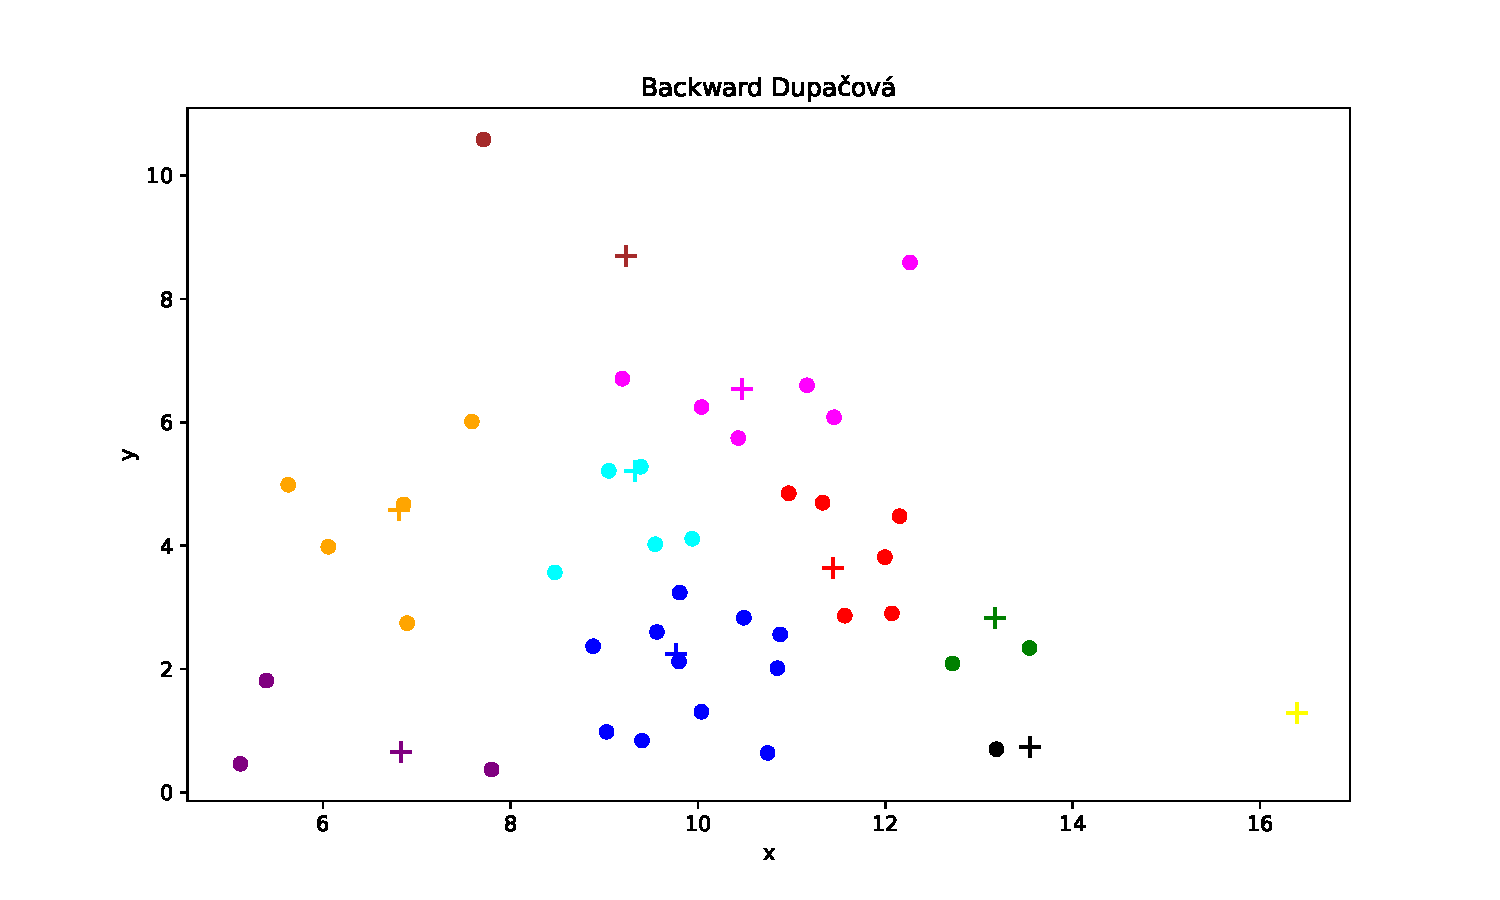
\includegraphics[width=\textwidth]{plots/dupacova backward.pdf}
        \caption{Output obtained with the backward algorithm}
        \label{result back}
    \end{subfigure}
    \hfill
    \begin{subfigure}[b]{0.45\textwidth}
        \centering
        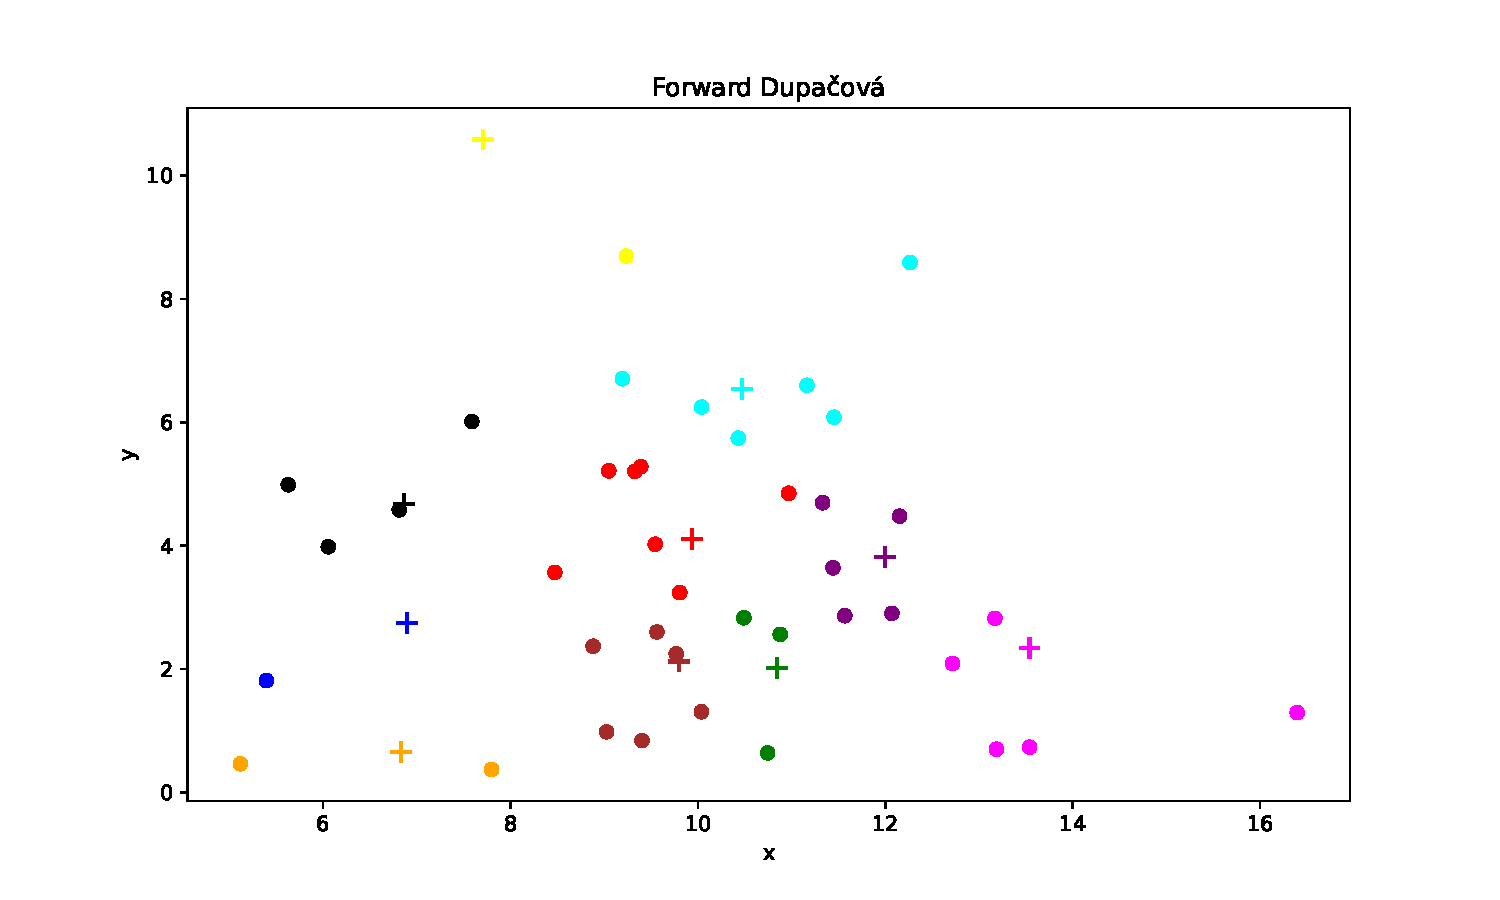
\includegraphics[width=\textwidth]{plots/dupacova forward.pdf}
        \caption{Output obtained with the forward algorithm}
        \label{result forw}
    \end{subfigure}
    \caption{Output visualization: forward and backward Dupačová et al' algorithm}
\end{figure}
Obviously outputs are not the same. Circles represent atoms and crosses represent atoms that are selected by an algorithm. A color represents a cluster. For the simulations to come, we'd rather use a bigger data-set in order to be more general. Every dimension should have a comparable data-range so that the distance between atoms isn't led by a single dimension. We will take samples of 3 normal distribution, 2 gamma and one uniform :
$$
\begin{pmatrix}
    \mathcal{N}\left(0,2\right) & \mathcal{N}\left(5,2\right) & \Gamma\left(0,2\right) & \Gamma\left(1,2\right) &\Gamma\left(2,2\right) & \mathcal{U}\left(0,10\right)
\end{pmatrix}^T.
$$

\subsubsection{Comparison}

\begin{figure}[ht]
    \centering
    \begin{subfigure}[b]{0.45\textwidth}
        \centering
        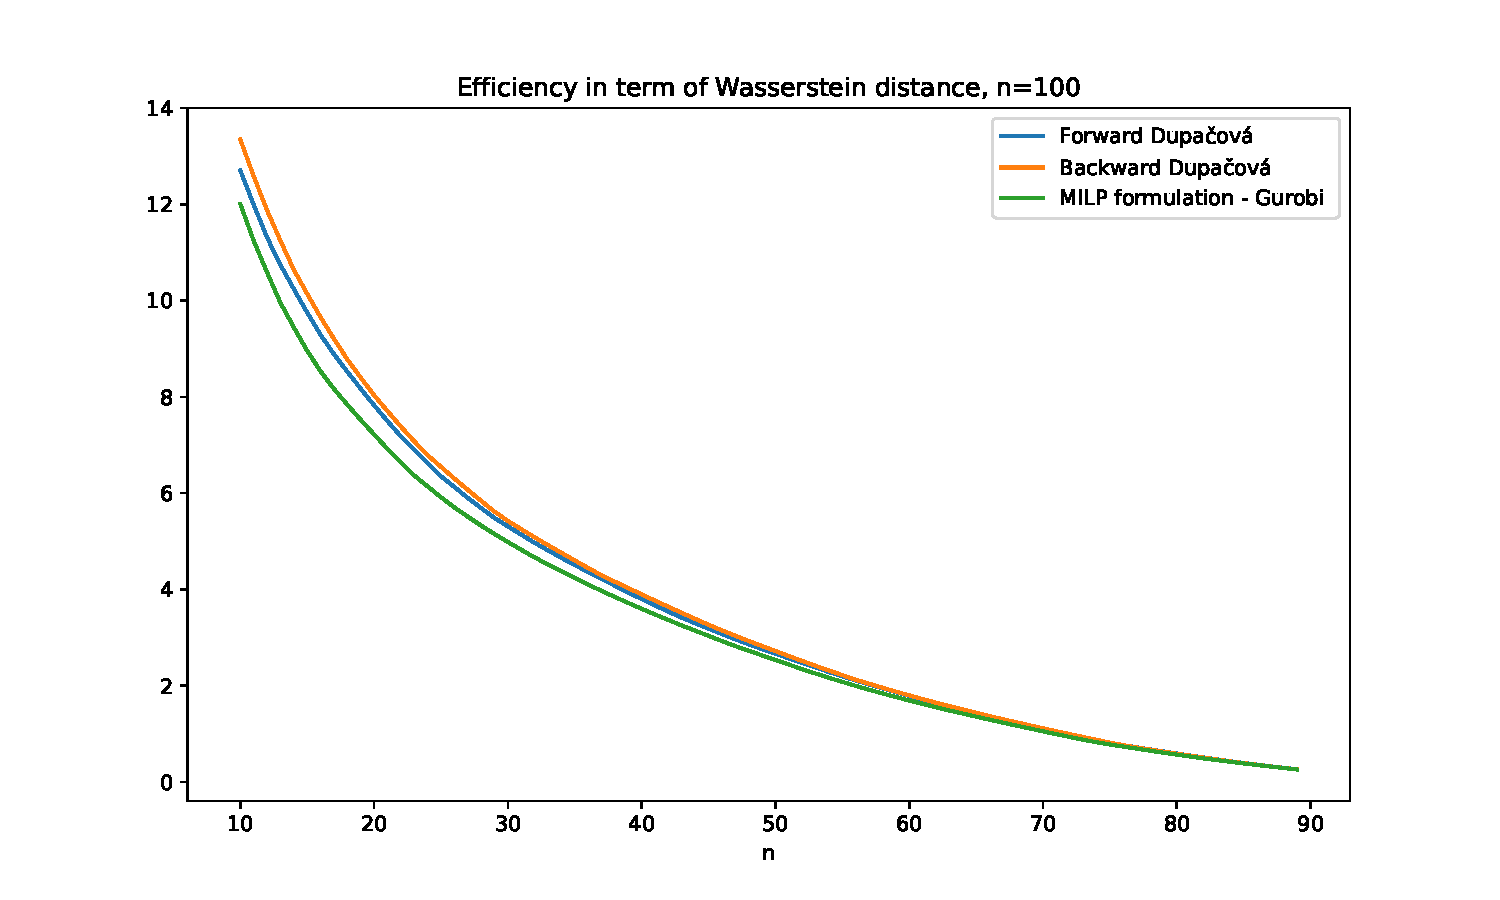
\includegraphics[width=\textwidth]{plots/efficiency milp.pdf}
        \caption{$d\left(P,Q\right)^2$ comparison between both algorithms}
        \label{dist for bac}
    \end{subfigure}
    \hfill
    \begin{subfigure}[b]{0.45\textwidth}
        \centering
        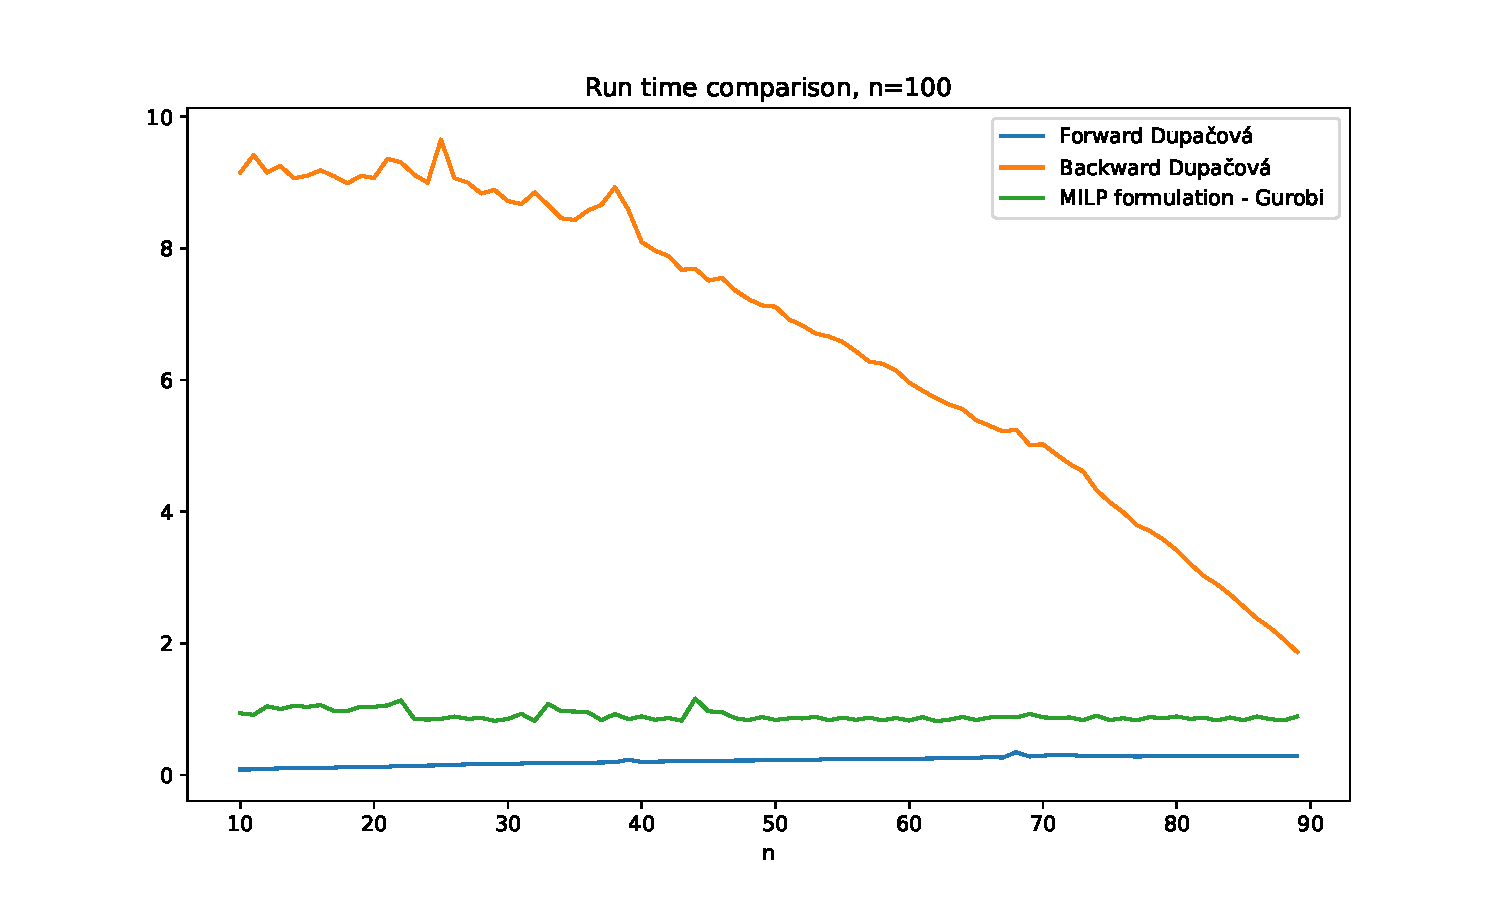
\includegraphics[width=\textwidth]{plots/run time milp.pdf}
        \caption{Run time comparison}
        \label{time for bac}
    \end{subfigure}
    \caption{Efficiency and calculation time comparison: forward and backward Dupačová et al' algorithm}
    \label{comparison dup}
\end{figure}

The horizontal axis of \Cref{comparison dup} represents $m$, the number of atoms in the reduced set. \Cref{dist for bac} shows that the efficiency in term of Wasserstein distance is similar and comparable for a reduced set obtained via forward or backward algorithm but still the forward method gets a slight lead. The main difference lies in CPU time, the efficient manner we found for the forward algorithm shows its advantages in \Cref{time for bac}, always below 0.05s whereas the backward algorithm can take up to one second and takes more time than the exact method. Forward algorithm has to be preferred when you're free to choose even when $m\approx n$. We solve the LP reformulation with Gurobi and it is very efficient, it is comparable to the forward method.\\
We have seen that backward method is not interesting in terms of CPU time. We will now compare forward method and MILP formulation for bigger distributions, it is $n\in\left[100,1000\right]$. Our goal is to understand the behaviours of both algorithms when $n$ increases. \ref{time for bac} may be irrelevant as Gurobi is very efficient with small-sized problems. Let us say we want to reduce a distribution with $n$ atoms to a distribution with $\frac{n}{4}$ atoms.

\begin{figure}[ht]
    \centering
    \begin{subfigure}[b]{0.45\textwidth}
        \centering
        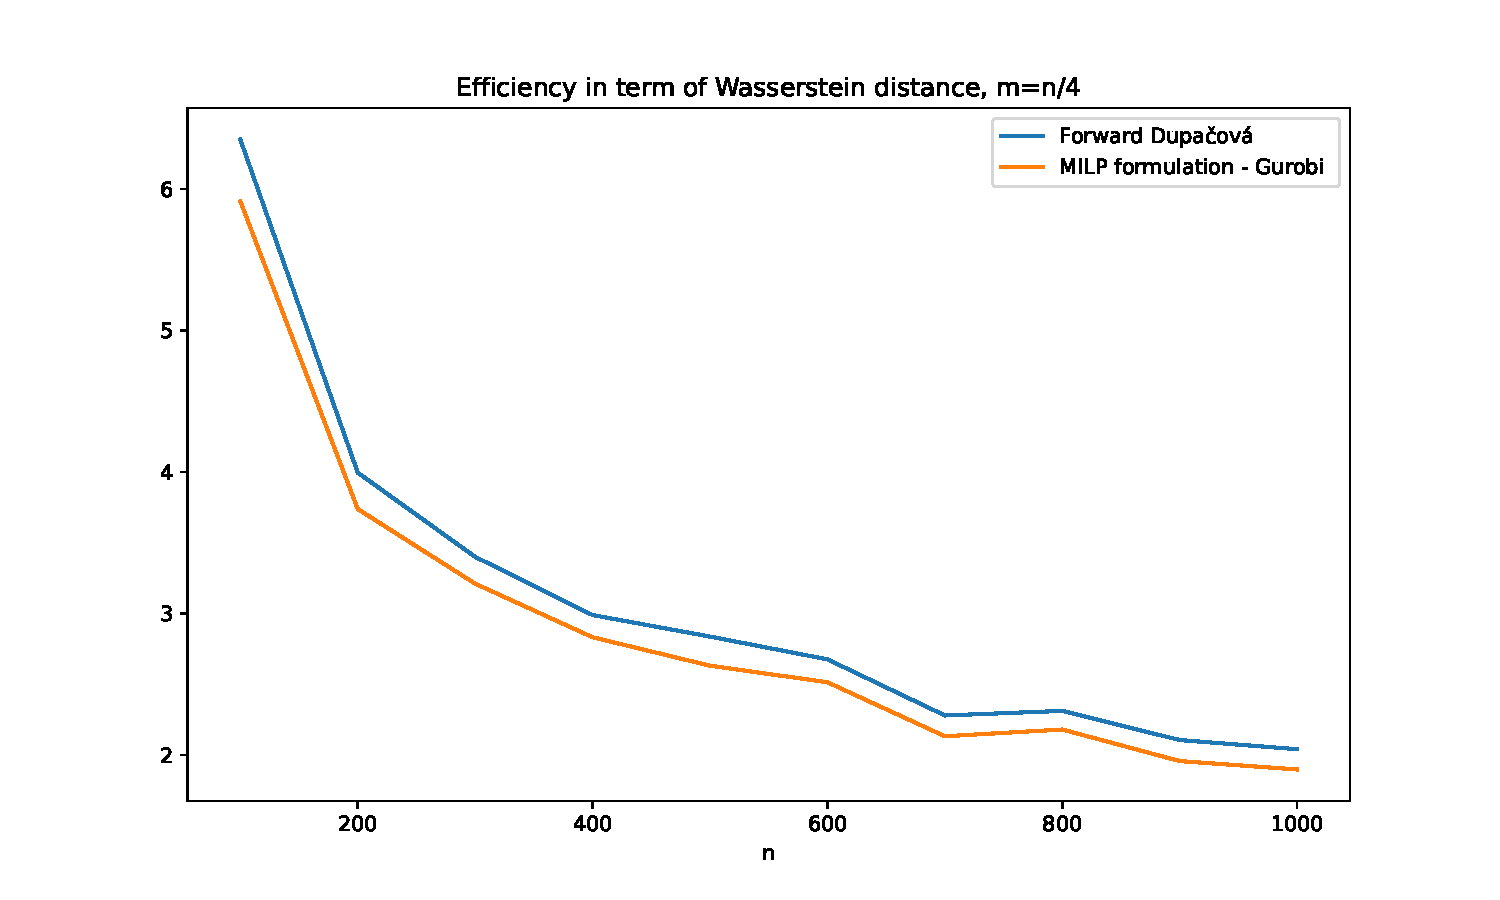
\includegraphics[width=\textwidth]{plots/milp efficiency n4.pdf}
        \caption{$d_2\left(P,R\right)^2$ comparison between both algorithms}
        \label{n4 effi}
    \end{subfigure}
    \hfill
    \begin{subfigure}[b]{0.45\textwidth}
        \centering
        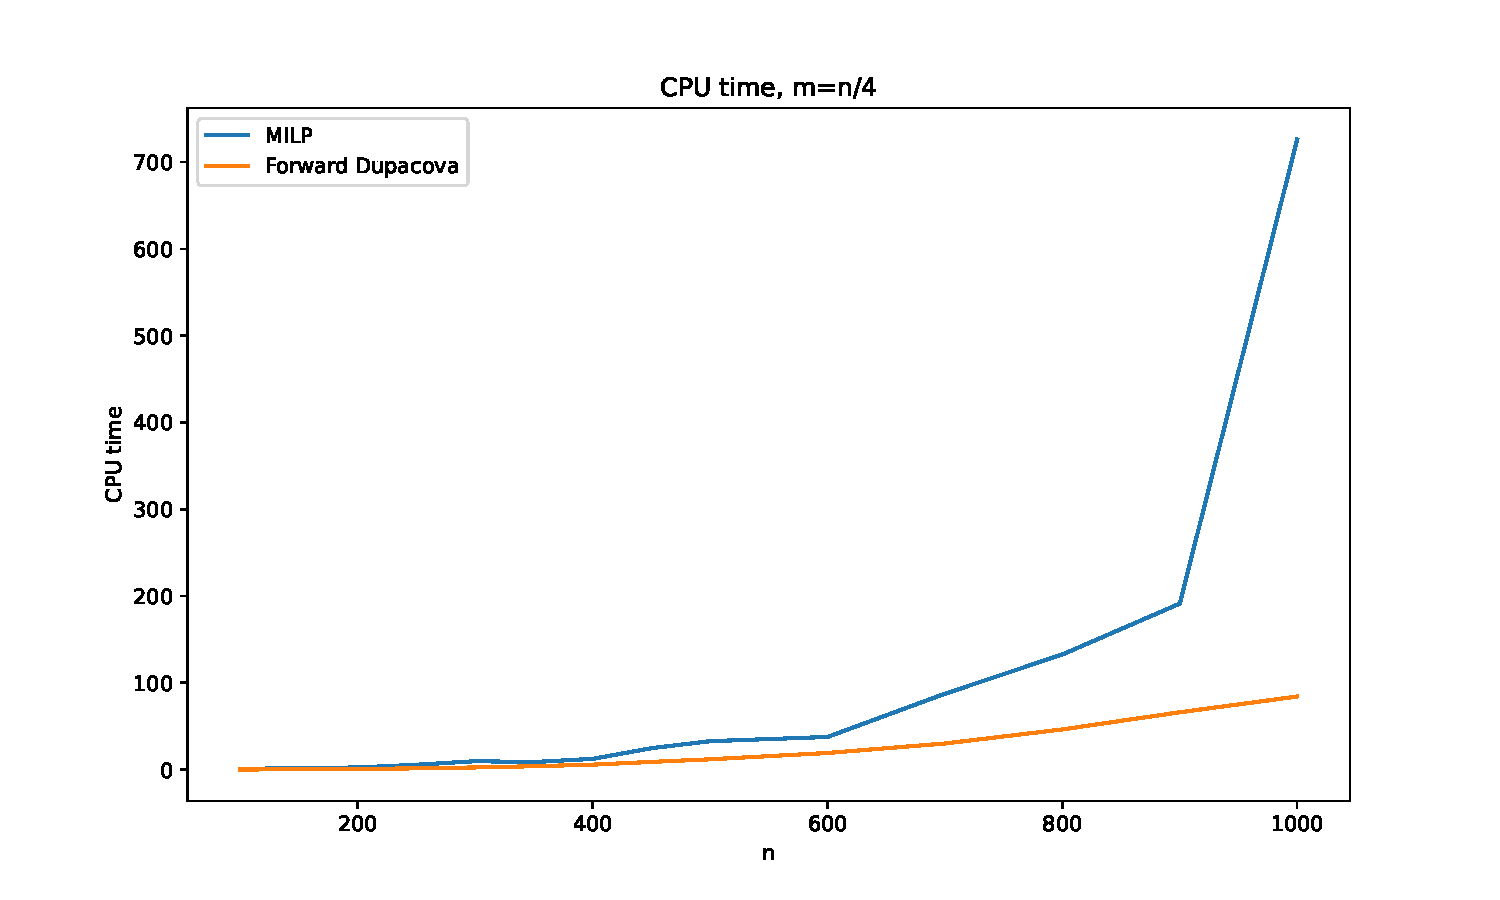
\includegraphics[width=\textwidth]{plots/run time comparison n4.pdf}
        \caption{Run time comparison}
        \label{n4 time}
    \end{subfigure}
    \caption{With a bigger $n$}
    \label{comparison n4}
\end{figure}

\Cref{complexity} tells us that forward method has a complexity of $\mathcal{O}\left(mn^2\right)$ what is meant to be far less than solving a LP. Gurobi may use heuristics or other sophisticated method to have this small run time gap. Without Gurobi the gap would be way bigger. Still there exists a huge gap in CPU time we can not neglect especially when $n$ grows. Behaviours in efficiency are not affected by this change of scale for $m$ and $n$.
\subsection{Local search}
A run of local-search is not assured to end in polynomial time. Thus it can be somehow long to compute with a random first guest of size $m$. The first comparison we have to make is between best-fit and first-fit method.
\subsubsection{Best-fit or first-fit}
Like Dupačová et al' algorithm, local-search will give you an approximate of $D_\ell\left(P,m\right)$ but local-search methods are meant to be more satisfying as they provide guarantees, see \ref{guarant}. First, we want to understand how the local search methods behave in comparison to the greedy algorithm and especially the forward method. In this part, the first guess $R$ of size $m$ is the $m$-first elements of the data-set, it is a random guess.

\begin{figure}[ht]
    \centering
    \begin{subfigure}[b]{0.45\textwidth}
        \centering
        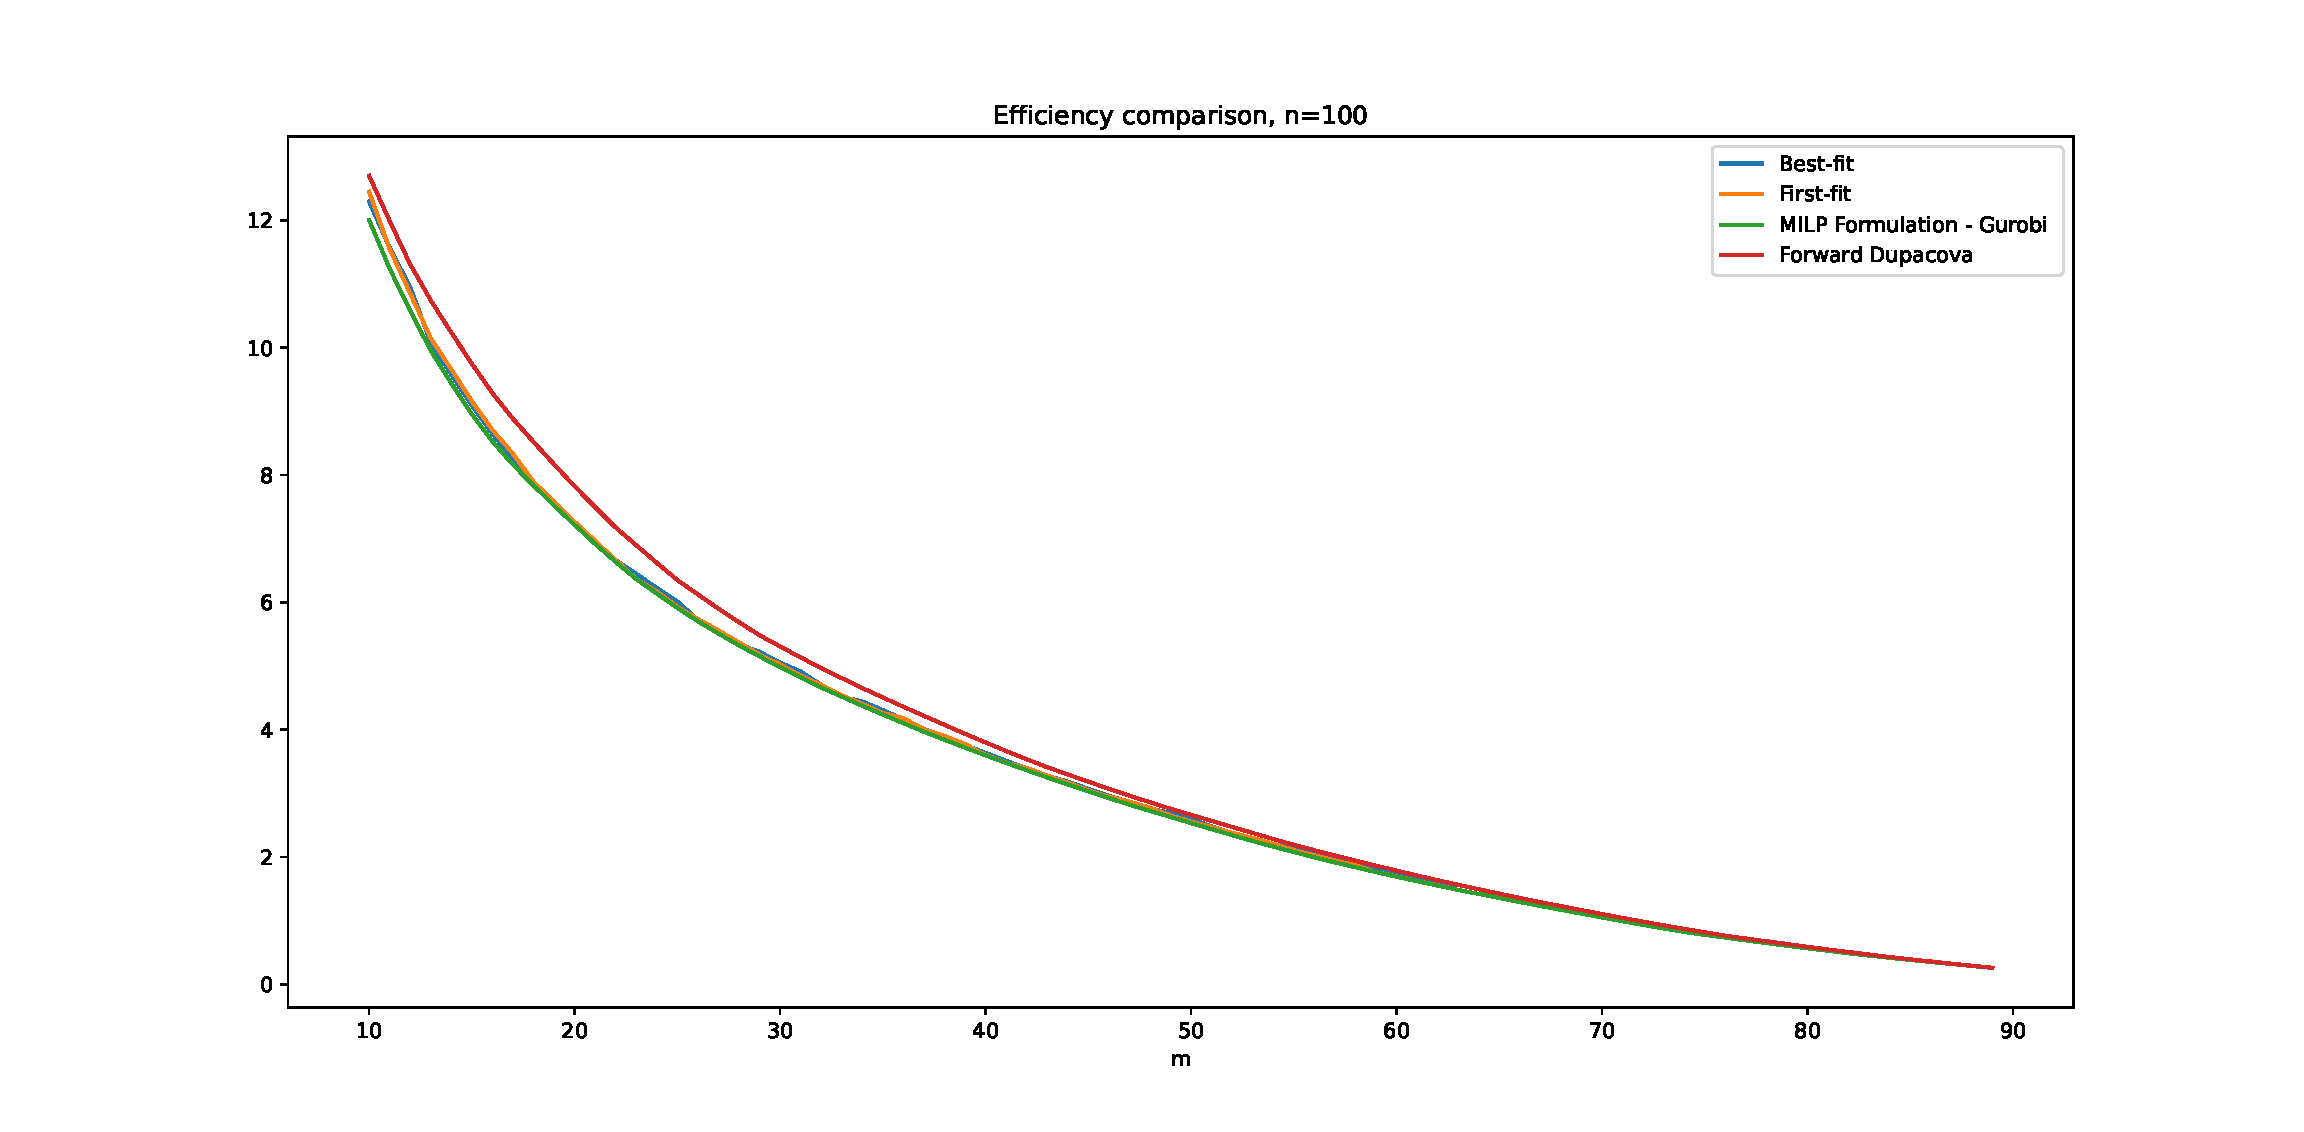
\includegraphics[width=\textwidth]{plots/milp local search efficiency.pdf}
        \caption{Efficiency comparison, local search and forward Dupačová}
        \label{value loc s}
    \end{subfigure}
    \hfill
    \begin{subfigure}[b]{0.45\textwidth}
        \centering
        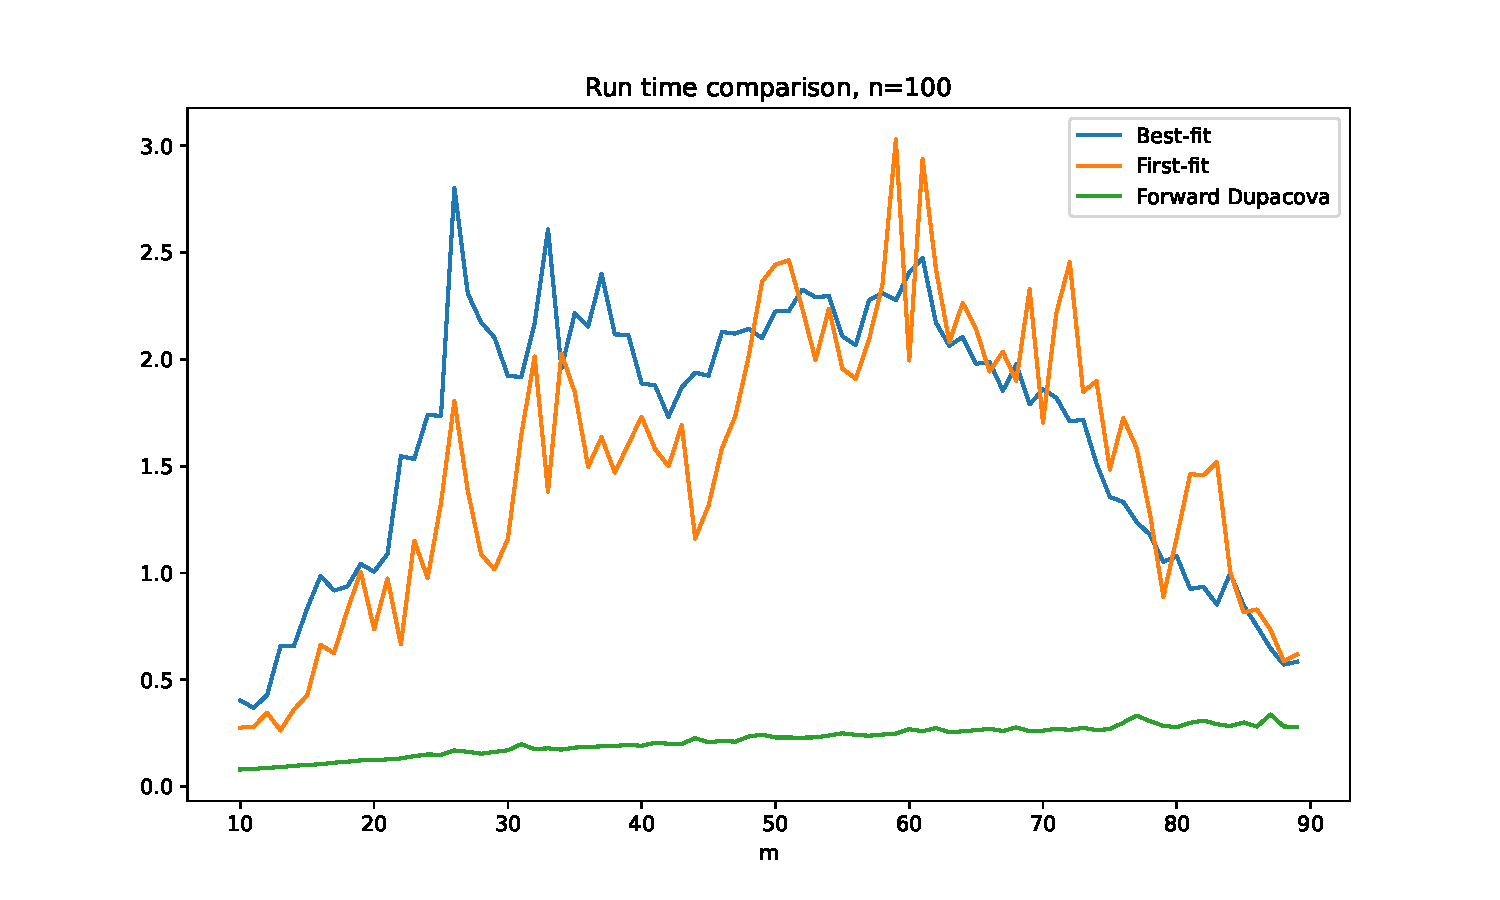
\includegraphics[width=\textwidth]{plots/run time local search.pdf}
        \caption{Calculation time comparison, local search methods and forward Dupačová}
        \label{time loc s}
    \end{subfigure}
    \caption{Efficiency and calculation time comparison: forward Dupačová and local search methods}
    \label{comparison loc}
\end{figure}

Run time grows linearly with $m$ with $n$ fixed for forward Dupačová et al' algorithm. For a run of local-search, as we do not know how many time we will enter the while loop for both local search methods, computation time looks messier for both method. Run time of the first-fit method tends to be even messier compared to best-fit method. Variability from $m$ to $m+1$ is bigger for the first-fit method. It aligns with the fact that best-fit is more stable as it compares all swap and chooses the best while first-fit swaps as soon as it finds an improvement \emph{even though it may be a very small one}, see \ref{step}. In terms of efficiency, both local-search methods give a better approximation than the one provided by forward Dupačová. As a mean, running a local search algorithm is 10 times longer than forward Dupačová.

In the following figure, we represent a ratio $r_m$ for $n=100$ and $m\in [\![10;90]\!]$. We define this ratio $r_m$ for a certain $m$ as: 
$$
r_m = \frac{d_\ell\left(P,Q\right)}{D_\ell\left(P,m\right)}.
$$
Where we know $D_\ell\left(P,m\right)$ thanks to the MILP formulation and $Q$ is generated with local-search or any other algorithm.

\begin{figure}[ht]
    \centering
    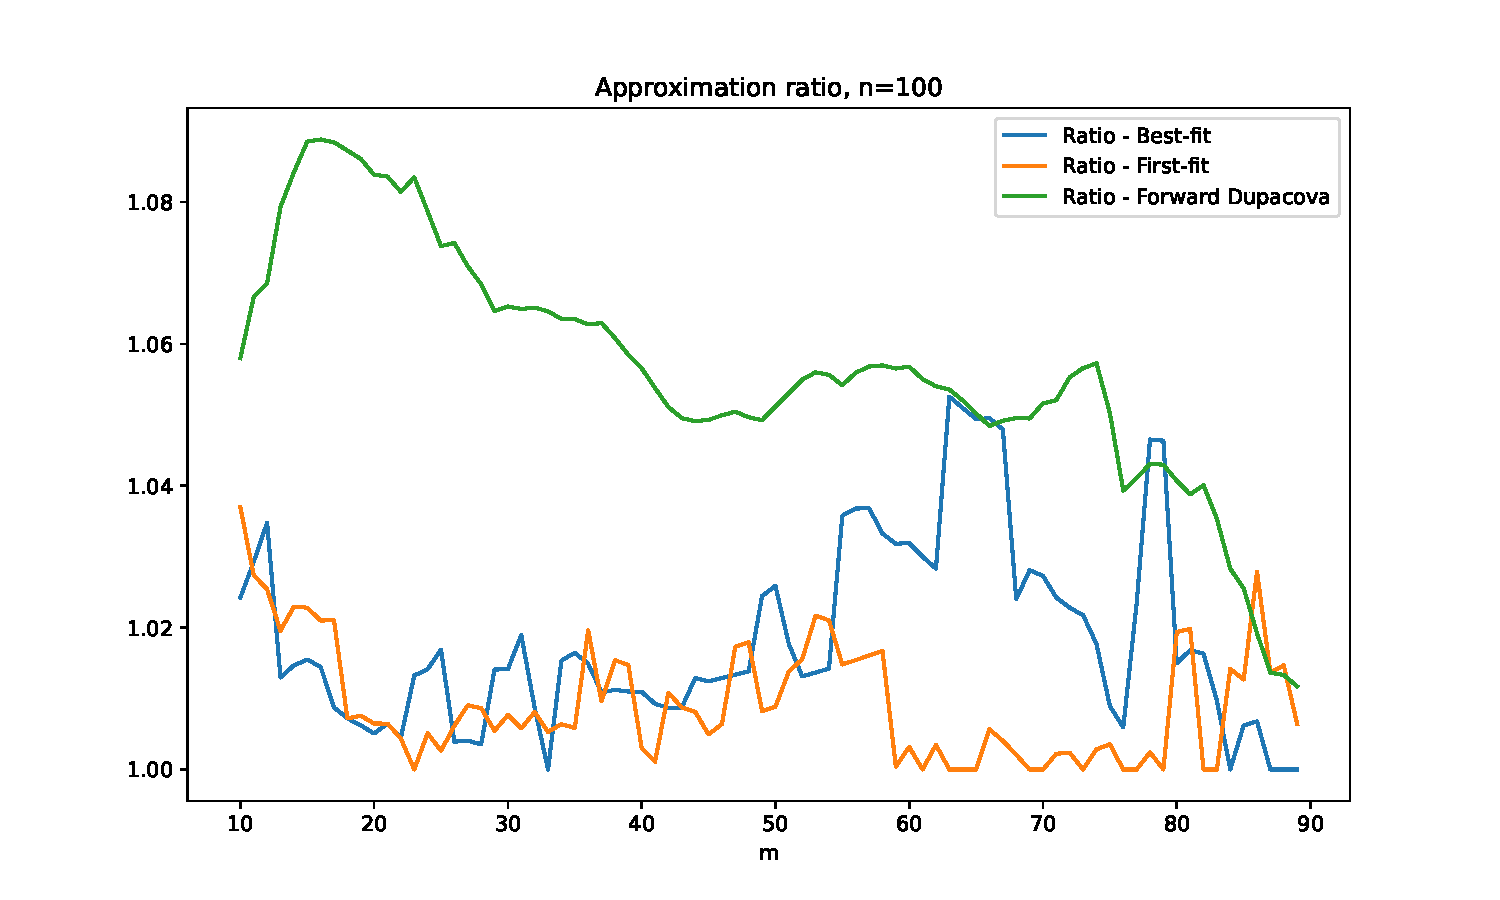
\includegraphics[width=0.45\textwidth]{plots/ratio with milp.pdf}
    \caption{Approximation ratio for $n=100$}
\end{figure}
    
\begin{figure}[ht]
    \centering
    \begin{subfigure}[b]{0.45\textwidth}
        \centering
        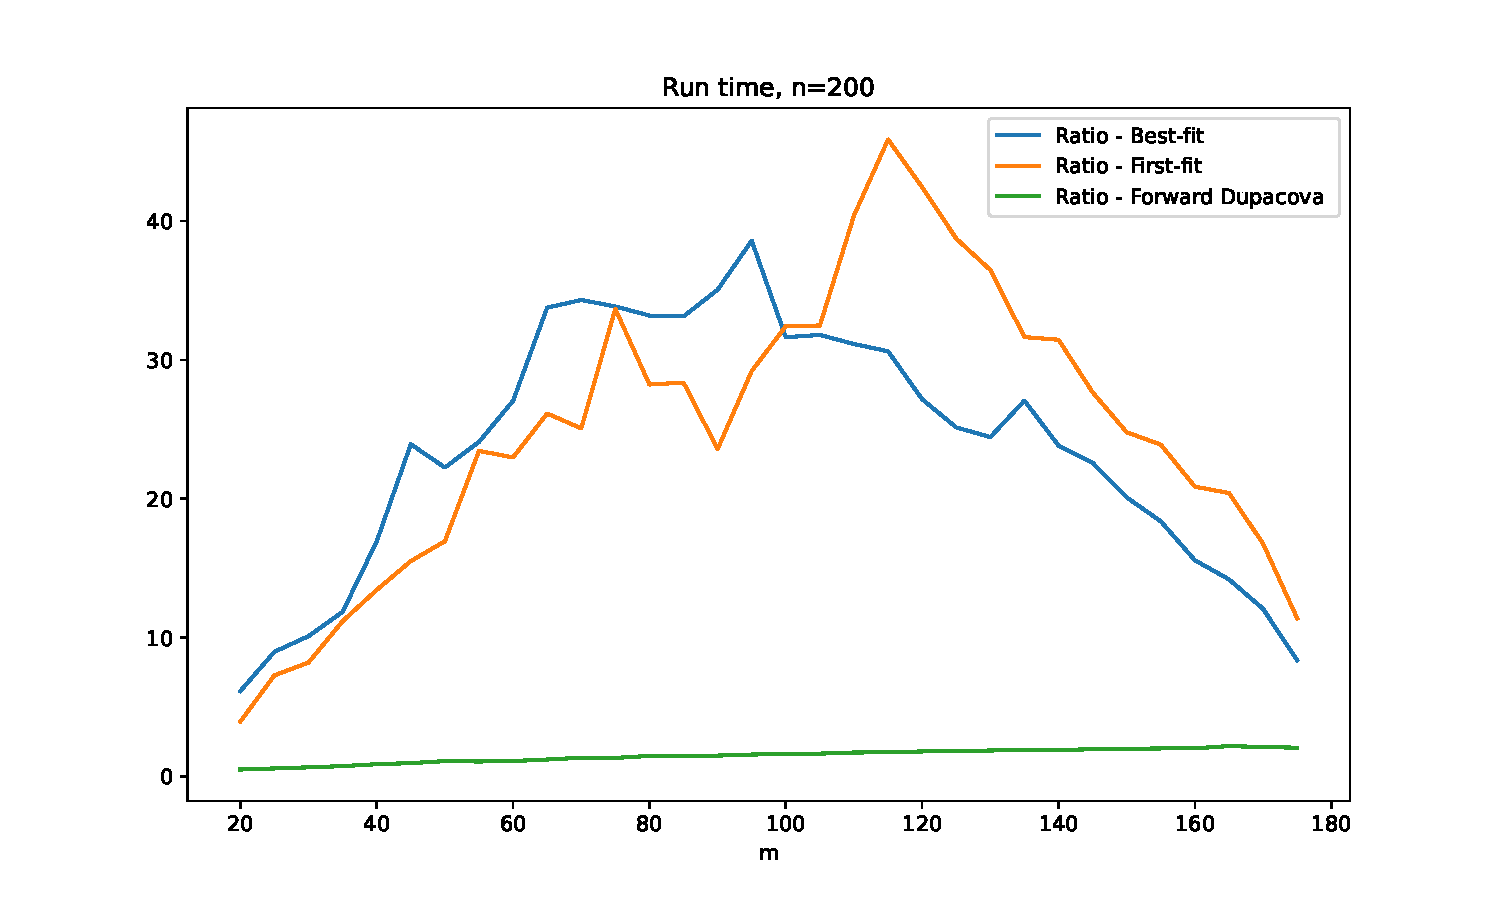
\includegraphics[width=\textwidth]{plots/run time 200.pdf}
        \caption{Run time for $n=200$}
    \end{subfigure}
    \hfill
    \begin{subfigure}[b]{0.45\textwidth}
        \centering
        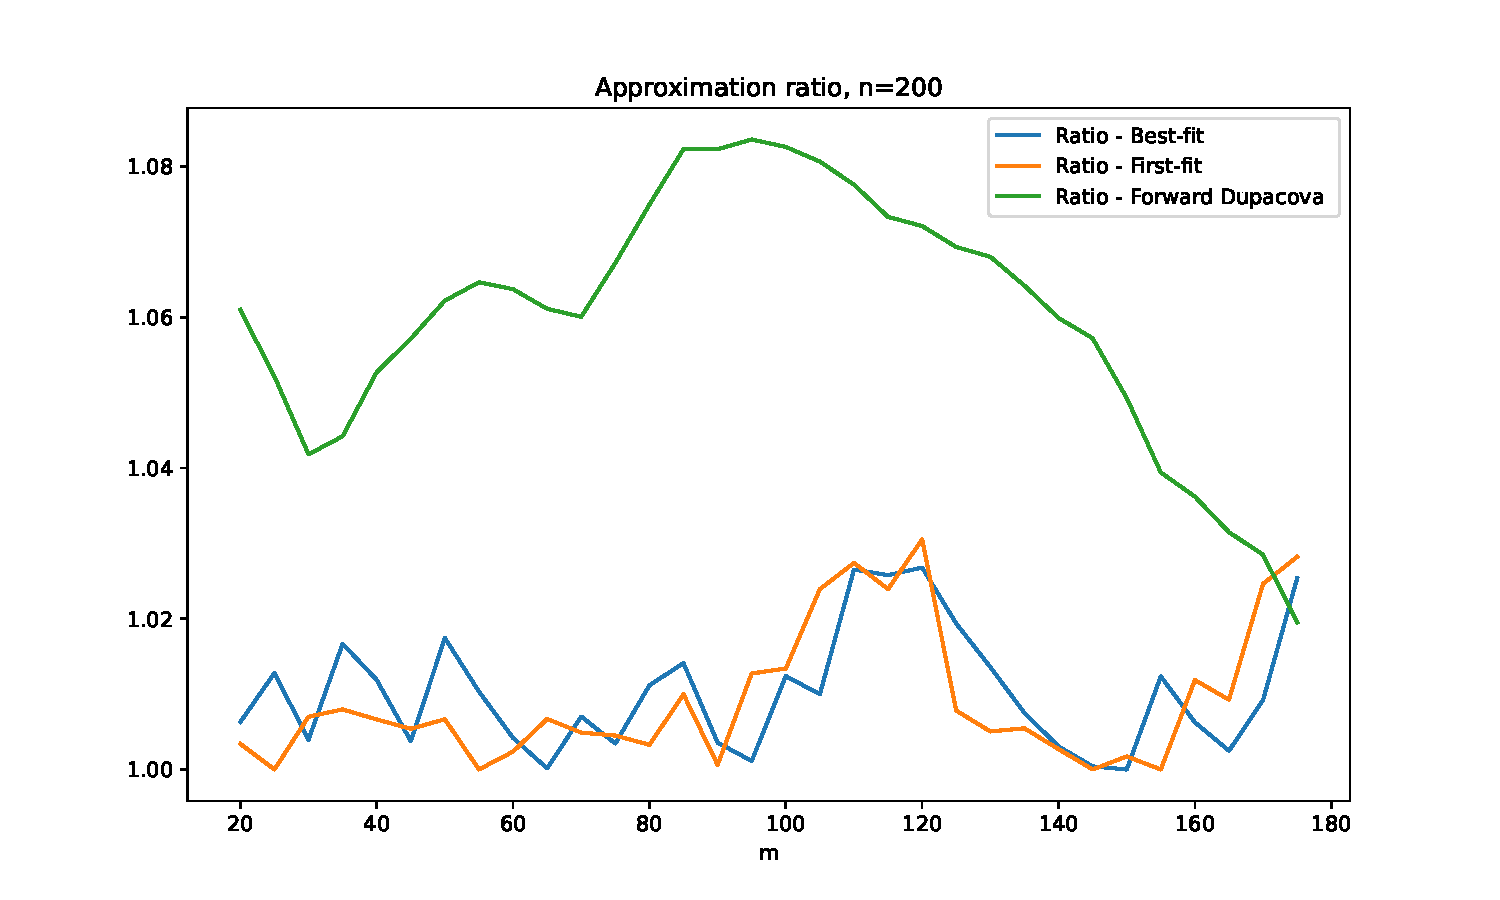
\includegraphics[width=\textwidth]{plots/ratio 200.pdf}
        \caption{Approximation ratio for $n=200$}
    \end{subfigure}
    \caption{Comparison for $n=200$ and variable $m$}
    \label{improvement ratio }
\end{figure}

For both $n=100$ and $n=200$, local-search gives a better approximation to $D_l\left(P,m\right)$ to the detriment of calculation time. Both best-fit and first-fit can be used even though the tendency is that first-fit has more run time variation from $m$ to $m+1$ when best-fit tends to be more stable. Best payouts for local-search are seen when you want to reduce $n$ to $m\leq\frac{n}{2}$. When $m\approx n$, there may still be a gain but thin. 

\subsubsection{Modified versions of local-search}
Local-search can be very excruciating but still we can play with different variables. E.g. not allowing small swaps for first-fit, use a clever set of starters. We will now present and compare variations of the local-search method with the aim of reducing run time without damaging efficiency. 
\paragraph{\textbf{Clever starters as a very first guess.}}
We decide to use the reduced set of size $m$ that we obtain with the forward Dupačová et al' algorithm, the backward algorithm and the set of of atoms that are the closest to the centroïds computed with a run of $m$-means on the data-set. The idea of this section is to compare efficiency and computation time between these methods and a random first guess. We will still compute the data-set as samples of the 6D data-set we have used so far. We can expect to reduce calculation time with an interesting starter $R$ of cardinal $m$ because it should lead to fewer changes in the local-search hence a lower run time. As order is important in first-fit, we will also use the reversed set obtained via forward Dupačová et al' algorithm. Using the reversed sequence of Dupačová et al' algorithm can be odd as the first atom of the reversed sequence will never be swapped but second, third, fourth are more likely to be changed as they weren't chosen at first, it is an idea we must consider. Inversely, the first atom chosen was the most centered so it gave a real direction to the choice that came later so changing this one would change a lot of things. Both ideas have their arguments that is why we must investigate. Note that best-fit for the original sequence or the reversed sequence must give the same output.

\begin{figure}[ht]
    \centering
    \begin{subfigure}[b]{0.495\textwidth}
        \centering
        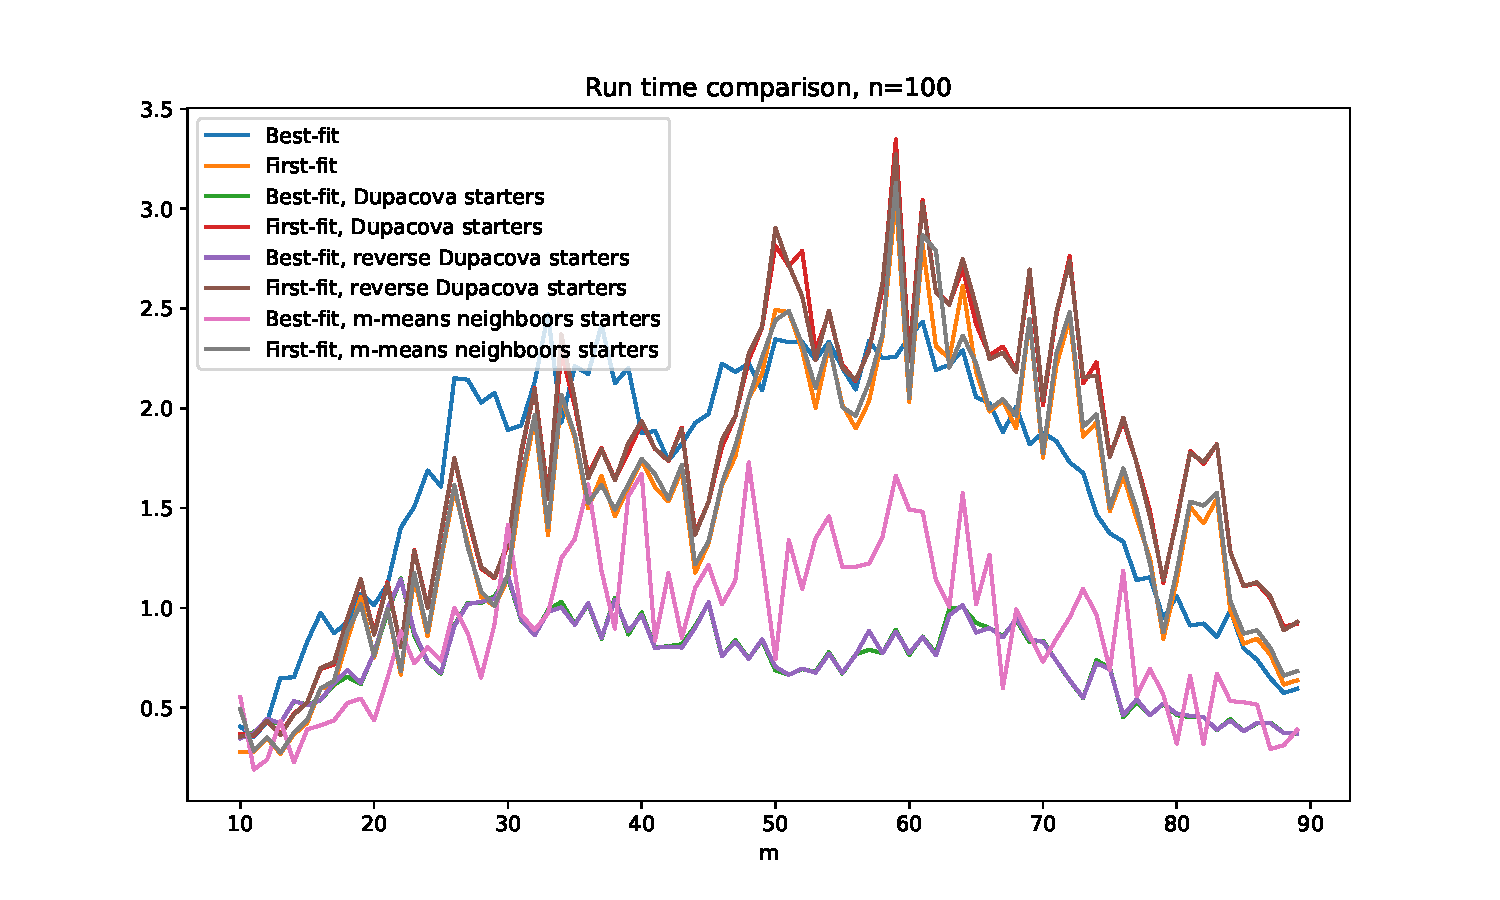
\includegraphics[width=1.1\textwidth]{plots/run time methods.pdf}
        \caption{Run time}
    \end{subfigure}
    \hfill
    \begin{subfigure}[b]{0.495\textwidth}
        \centering
        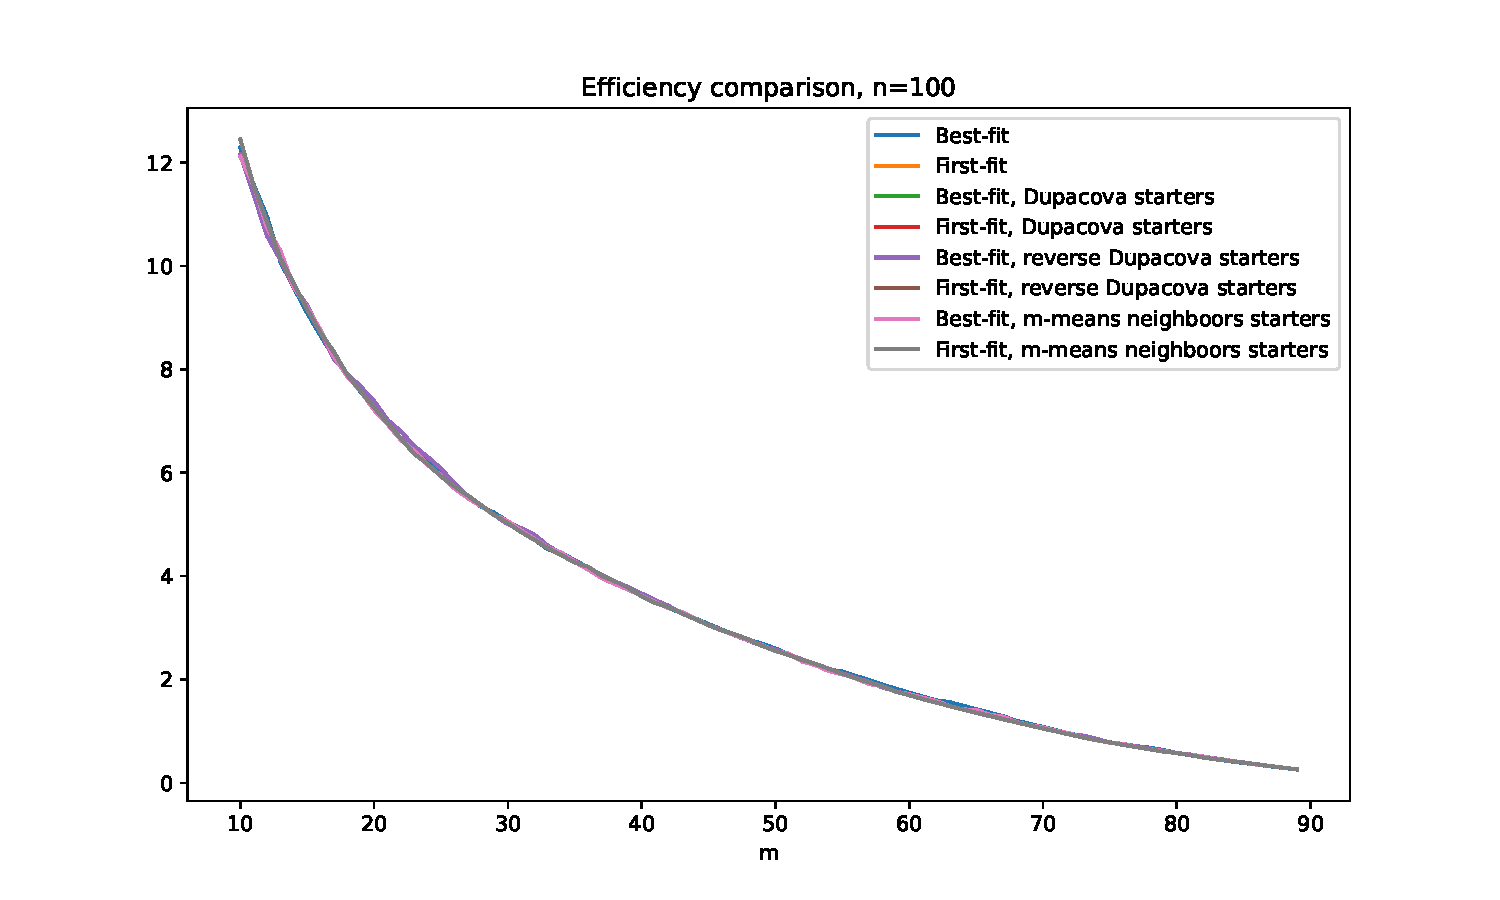
\includegraphics[width=1.1\textwidth]{plots/value methods.pdf}
        \caption{Efficiency}
    \end{subfigure}
    \caption{Comparison of local-search variants}
    \label{methods}
\end{figure}

\Cref{methods} is satisfying because all methods we proposed reduce run time in general and sometimes by more than a factor 5. Best methods to consider are best-fit with Dupačová starters (reverse or not it does not matter), first-fit with Dupačová starters and best-fit with $m$-means neighbours starters. Efficiency is similar for all methods what is relieving. 

\paragraph{\textbf{First-fit with a minimum step.}}\label{step}
First-fit method lacks of efficiency. An idea is to reduce run time by allowing only changes that reduce sufficiently the cost function. Meaning that the swap is accepted if and only if: $$
d_\ell\left(P,Q_{i+1}\right) \leq d_\ell\left(P,Q_i\right) - \epsilon.
$$
Where $Q_i$ was the distribution before iteration and $Q_{i+1}$ a distribution we are testing with one swap compared to $Q_i$. The idea of this part is to find an interesting $\epsilon$ to allow efficiency in a first-fit method. To be general and not to rely on a specific problem, we are testing $\epsilon$ as: $$\epsilon=pd_\ell\left(P,D\right),$$ with $p$ a parameter that has to be defined and $d_\ell\left(P,D\right)$ the distance between the original distribution $P$ and $D$ the distribution given by the forward Dupačová et al' algorithm. We will compare run time and efficiency in terms of $p$:

\begin{figure}[ht]
    \centering
    \begin{subfigure}[b]{0.495\textwidth}
        \centering
        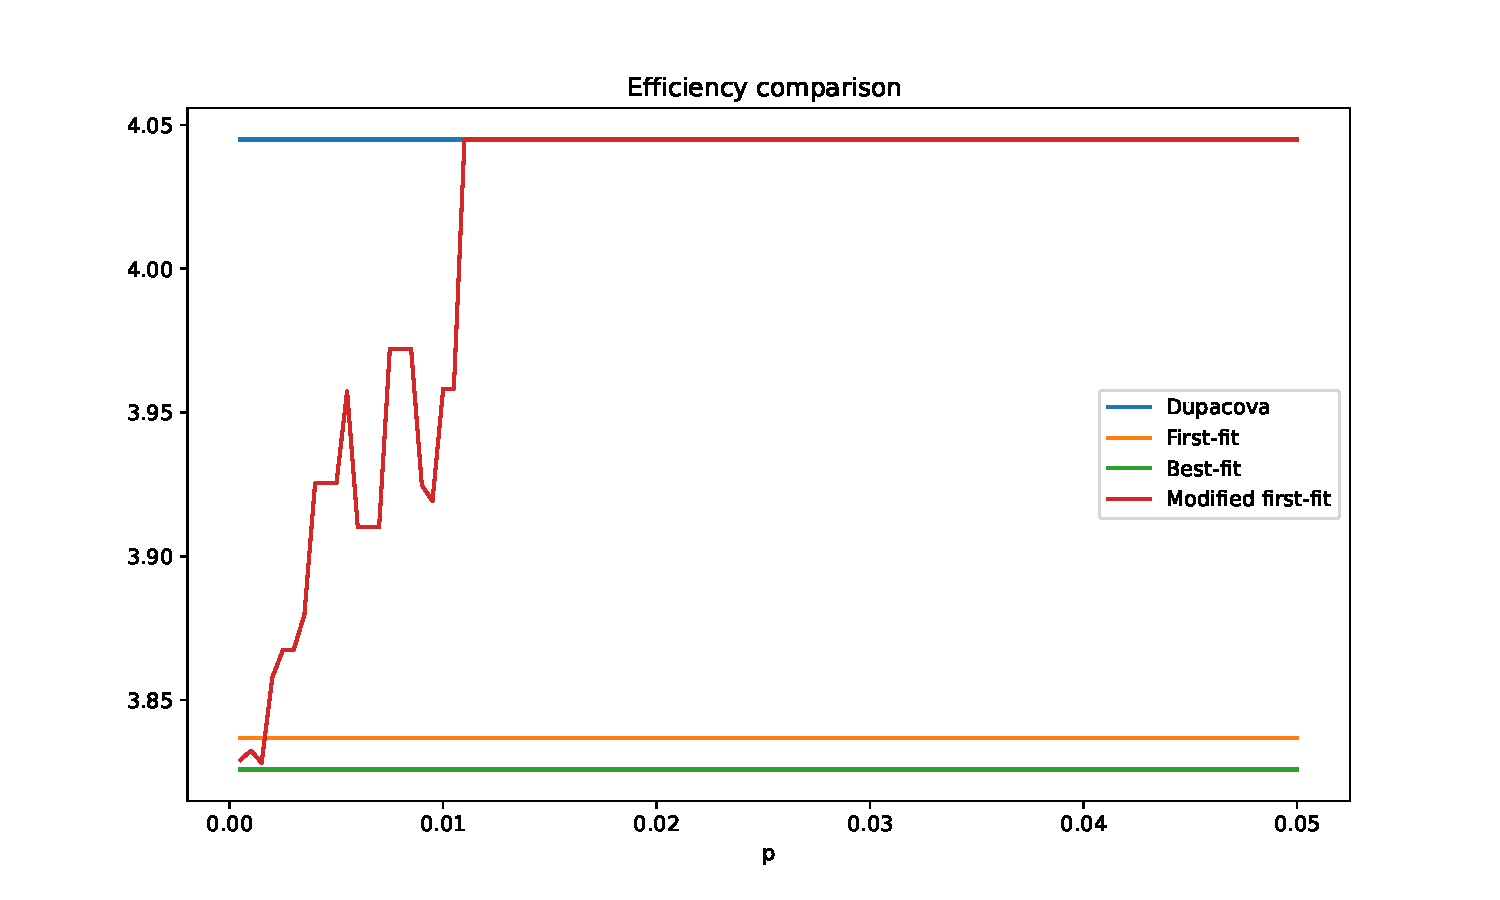
\includegraphics[width=1.1\textwidth]{plots/efficiency p.pdf}
        \caption{Efficiency}
    \end{subfigure}
    \hfill
    \begin{subfigure}[b]{0.495\textwidth}
        \centering
        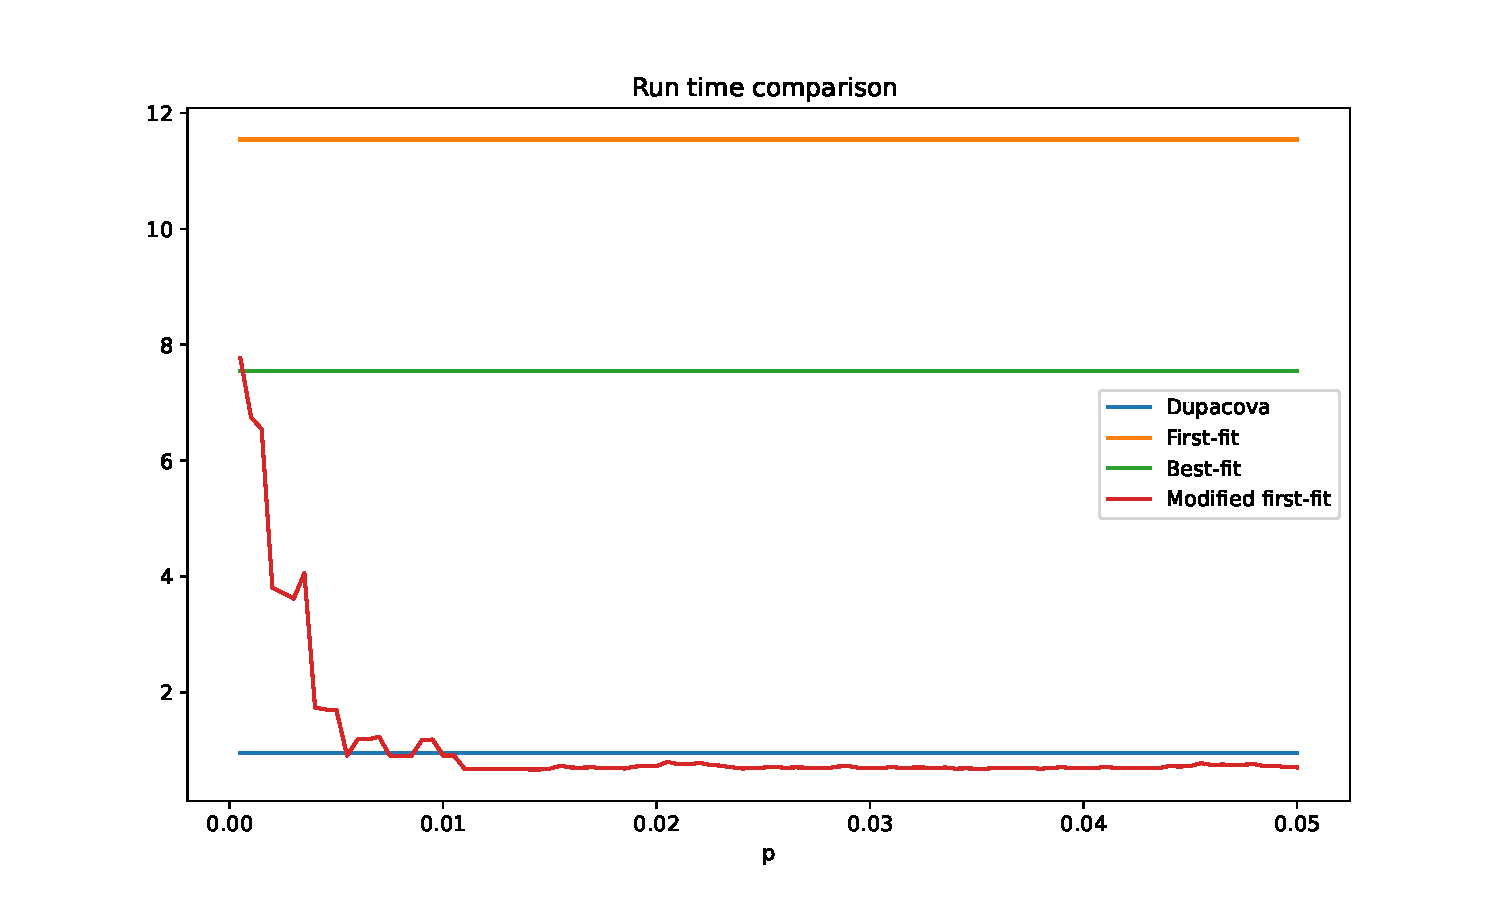
\includegraphics[width=1.1\textwidth]{plots/run time p.pdf}
        \caption{Run time}
    \end{subfigure}
    \caption{Comparison, $n=200$, $m=50$}
    \label{p}
\end{figure}

Both figures are saying that we must study this algorithm in the range $p\in\left]0,0.015\right]$, where it grants a lower run time and a better output than Dupačová.  \rp{là}

\begin{figure}[ht]
    \centering
    \begin{subfigure}[b]{0.495\textwidth}
        \centering
        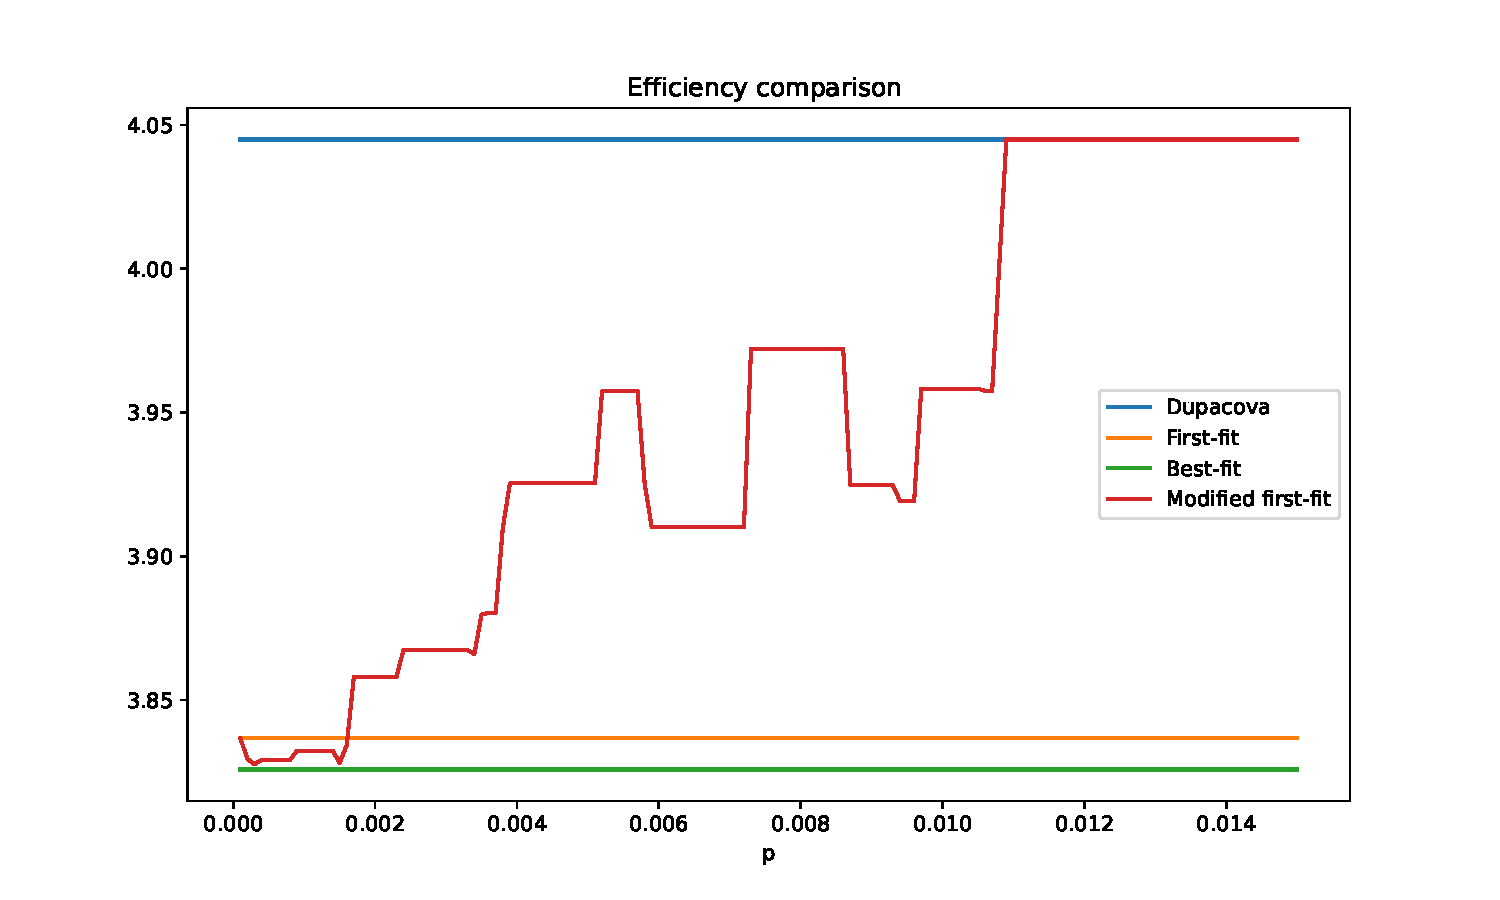
\includegraphics[width=1.1\textwidth]{plots/efficiency small scale p.pdf}
        \caption{Efficiency}
    \end{subfigure}
    \hfill
    \begin{subfigure}[b]{0.495\textwidth}
        \centering
        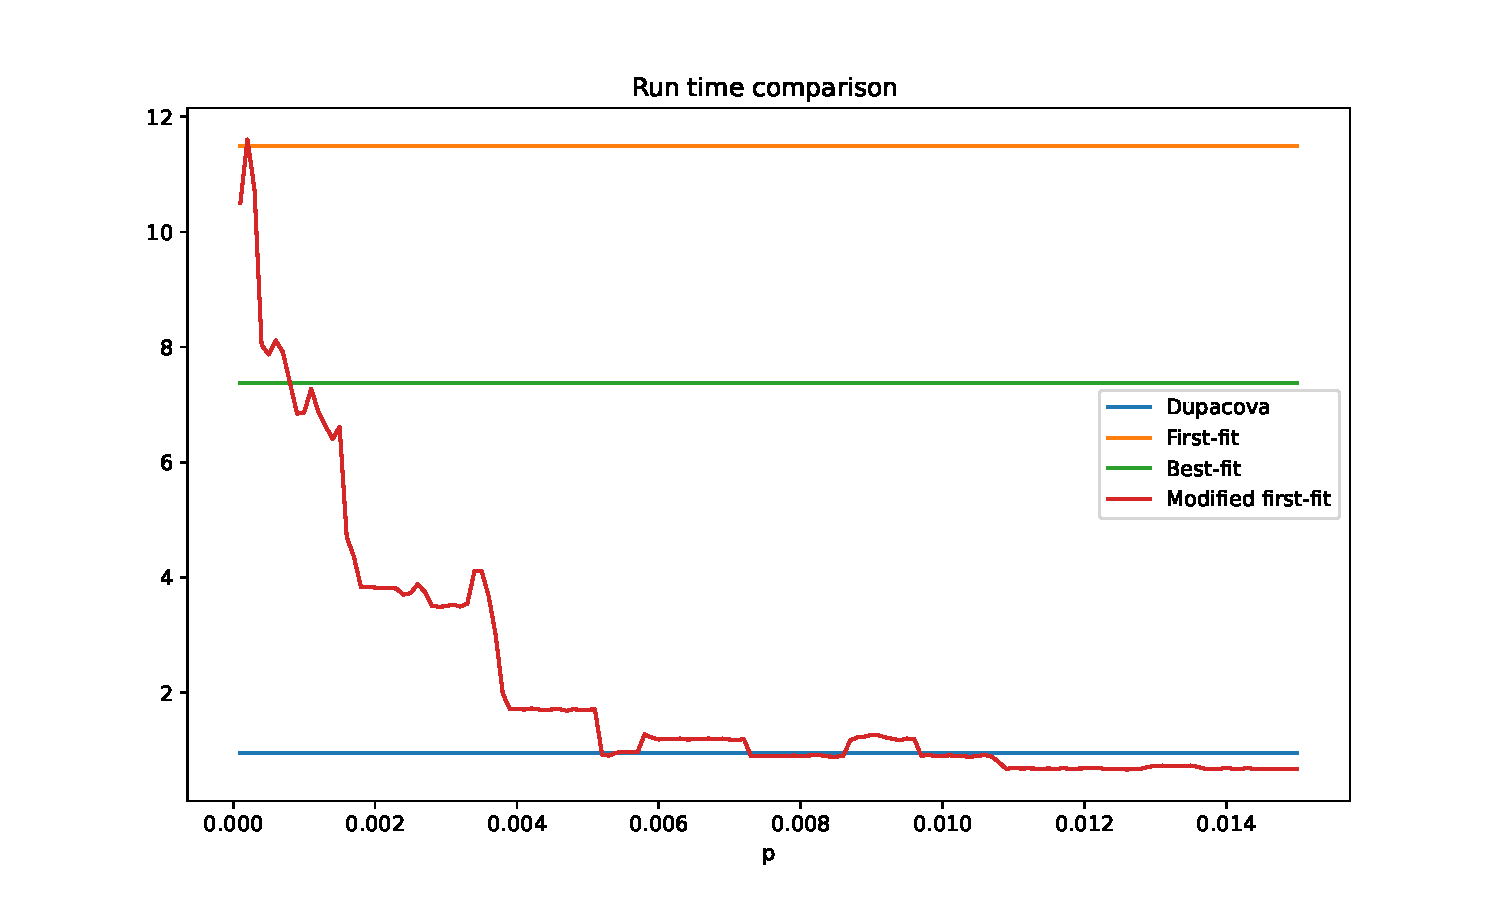
\includegraphics[width=1.1\textwidth]{plots/RUN TIME p small scale.pdf}
        \caption{Run time}
    \end{subfigure}
    \caption{Comparison, $n=200$, $m=50$, scale of interest}
    \label{p small scale}
\end{figure}

An interesting remark would be to say that with $p\approx 0.001$, this method even gives a better approximate to $D_\ell\left(P,m\right)$ than the original first-fit meaning $p=0$. Still this remark exists for a particular distribution here maybe we can not assume that statement in general. When $p$ increases, run time reduces as well as efficiency. Through the existence of the parameter $p$ this method provides a \emph{continuous transformation} of the space between the approximation of $D_\ell$ by Dupačová et al' algorithm and local-search. \rp{mettre en avant cette remarque à mon avis c'est important}

\clearpage
\paragraph{\textbf{Using randomization in first-fit.}}
The first-fit method relies on a linear exploration of the current solution until you find an improvement. Exploring the current solution always with the same method can lead to a lot of useless calculation, e.g. if you know that you only have to swap either the last atom or the one before but you explore linearly the current solution. The idea is to change the exploration order by introducing a random shuffle so that the exploration order is never the same. In order to generate these permutations, we use the algorithm of Fisher-Yates, this algorithm generates a permutation of $n$ elements in a linear run time, all permutations being equally probable.
\begin{algorithm}\caption{Fisher-Yates algorithm}\label{fisher yat}
    \For{$i$ from $n-1$ down to $1$}{
    $j\gets k$, $k$ randomly chosen in $ [\![0,i]\!]$  \\
    Exchange the value in $i^{\text{th}}$ position with the one in $j^{\text{th}}$.}
\end{algorithm}
For this simulation we use $n=100$, $m$ as the $x$-axis and  starters. Note that we run 25 times the random first-fit method to get the plot "mean random first-fit"
\begin{figure}[ht]
    \centering
    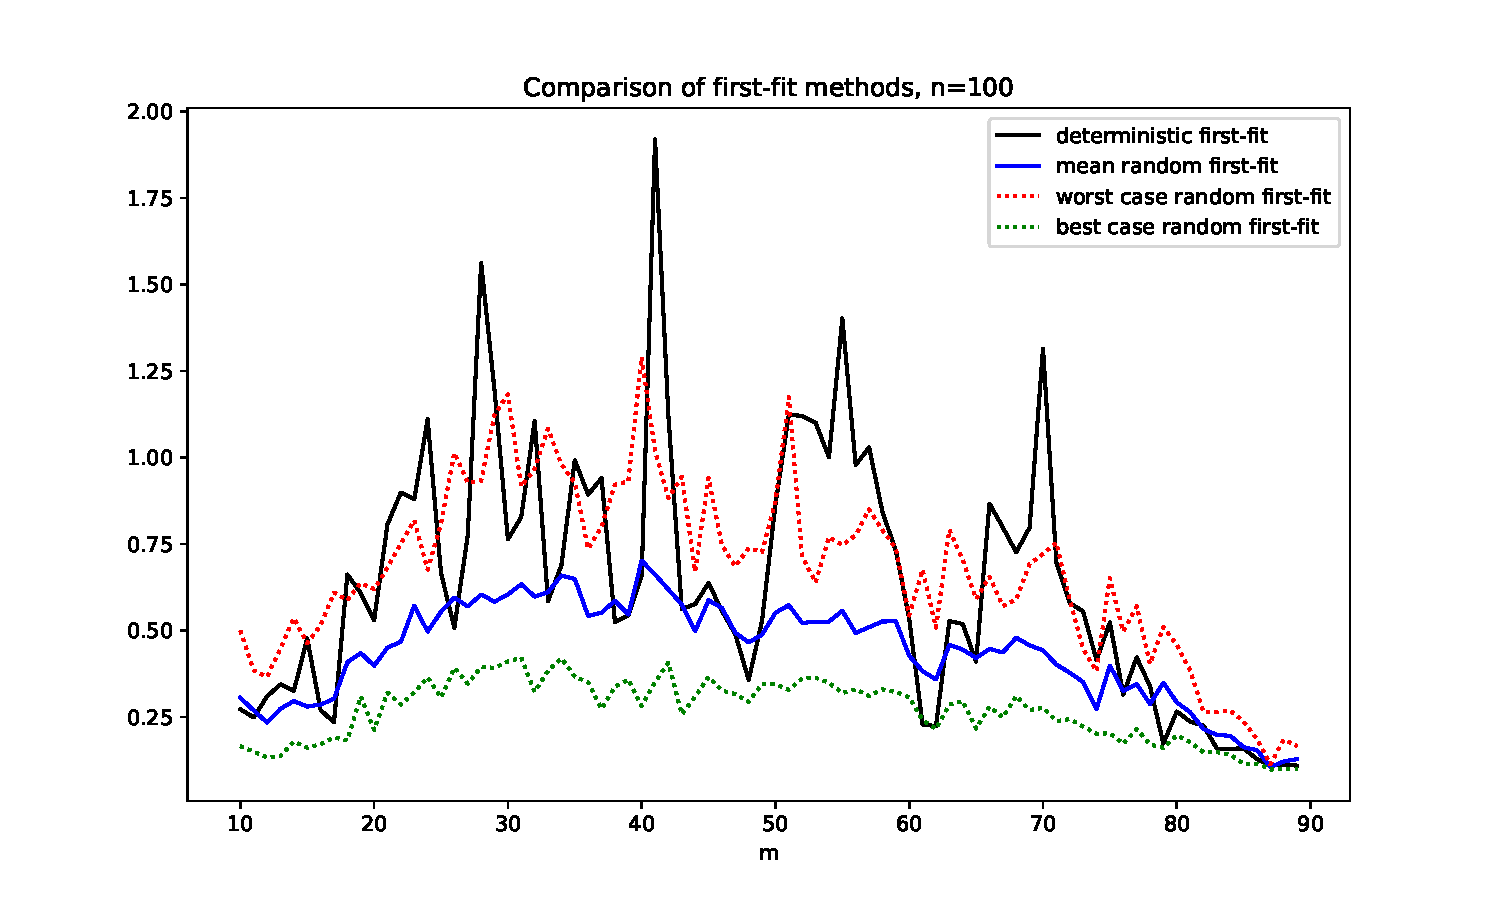
\includegraphics[width=0.5\textwidth]{plots/random first fit.pdf}
    \caption{Random first-fit results}
    \label{random ff}
\end{figure}
Using this randomized order helps us to gain stability in run time. Even the worst case of this randomized method is generally better or at least comparable to the deterministic first-fit. There is a clear gain. If the randomization procedure was $\mathcal{O}\left(1\right)$ the gain would have been even better because this procedure adds one more stage in the algorithm. The gain in run time seems to be huge for a small $m$, when $m\approx n$, this procedure does not seem to be a good idea.

\subsection{Fusion of local search and $m$-means}
In this part we want to compare \Cref{improved ls}  with a generalized $m$-means for an approximation of $C_l$ as proposed in \Cref{k m} and \Cref{Local search}. For the sake of run time and thanks to the above analysis, we will use the best-fit method with Dupačová starters whenever we need to run a local-search. We will only optimize on the centroïds once meaning that we compute the reduced set with a run of local-search and then we reoptimize on the centers, $y_j^*=\text{mean}\left(I_j\right)$ because we work with the euclidian distance and $\ell=2$.


\begin{figure}[ht]
    \centering
    \begin{subfigure}[b]{0.495\textwidth}
        \centering
        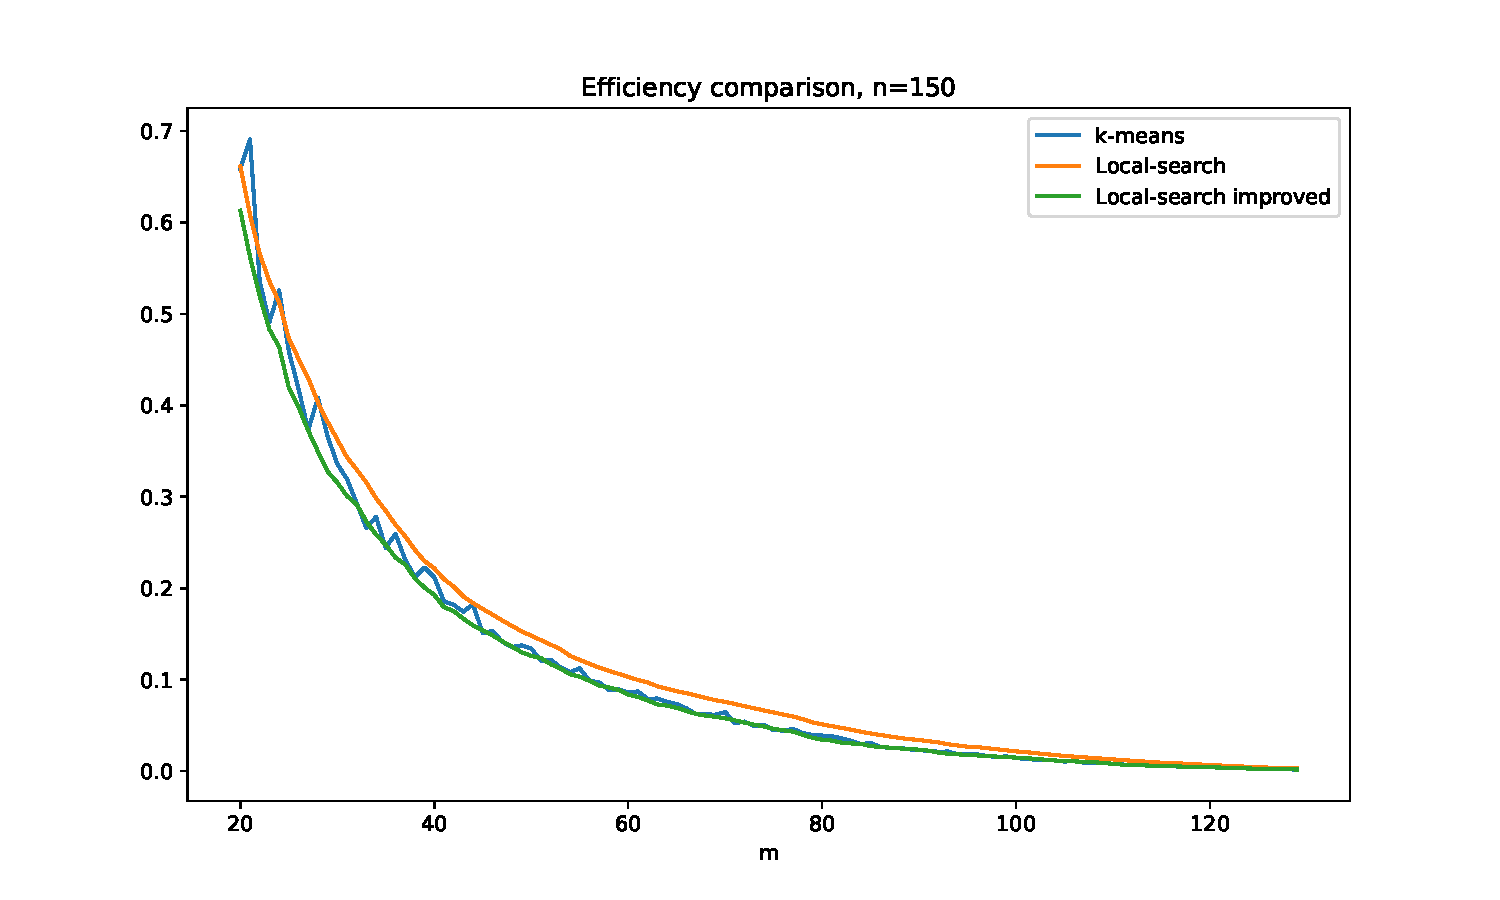
\includegraphics[width=1.1\textwidth]{plots/effiency cl.pdf}
        \caption{Efficiency}
    \end{subfigure}
    \hfill
    \begin{subfigure}[b]{0.495\textwidth}
        \centering
        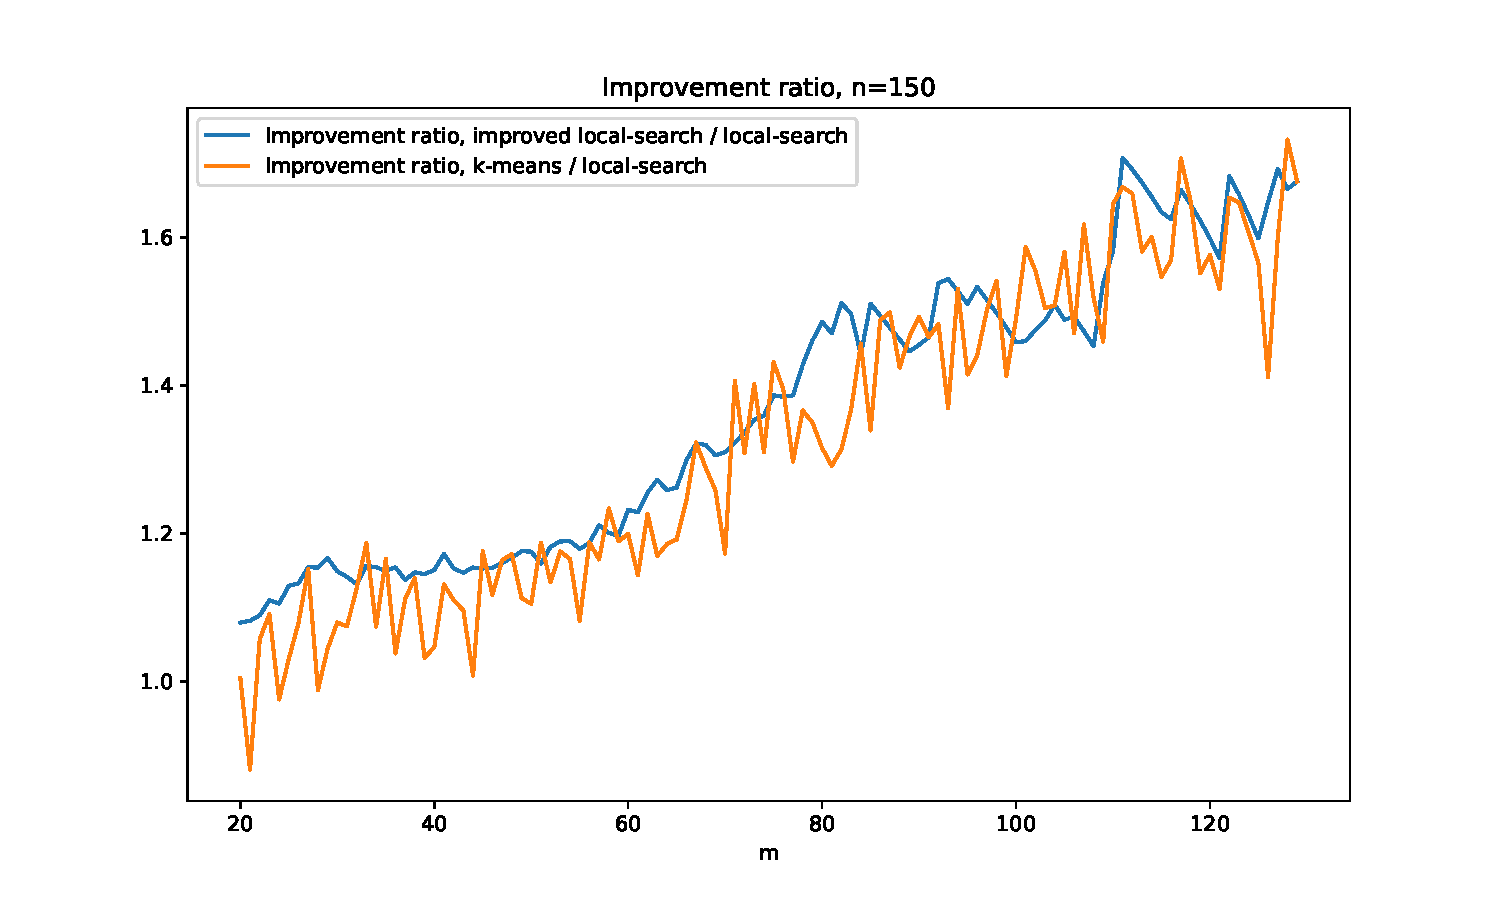
\includegraphics[width=1.1\textwidth]{plots/efficiency ratio cl.pdf}
        \caption{Improvement ratio}
    \end{subfigure}
    \caption{Efficiency comparison, $n=150$}
    \label{cl }
\end{figure}


The $m$-means algorithm tends to be a little better than local-search in this simulation even though its approximation ratio is not bounded. Nevertheless, it remains understandable to have a closer distribution with $m$-means because it can decide to use atoms that are not included in $\text{supp}\left(P\right)$. Combining the idea of $m$-means with local-search gives in general a slightly better value and most important it presents more stability and by stability I mean that the efficiency curve is smoother.

\section{The multiproduct assembly problem}
In this section, we will apply scenario reduction to the \emph{multiproduct assembly problem} with finitely many demand scenarios. This assumption can be allowed as the manufacturer may use $k$ past demands with a probability $\frac{1}{k}$ to model the future demand.
\subsection{Problem}
\cite[Chapter 1.3]{shapiro_lectures_2009} gives a clear presentation of the problem that I am writing, I will be adding notes when necessary. A manufacturer produces $n$ \emph{products}. Each product is composed by \emph{parts}. There are $m$ parts. The product $i$ requires $a_{ij}$ units of part $j$, then $a_{ij}\in\mathbb{N}$. Demands are modeled as a random vector $D=\begin{pmatrix} D_1 & \hdots & D_n \end{pmatrix}$ note that the distribution of $D$ is known. Before the demand is known the manufacturer may preorder parts at a unit cost of $c_j$ for a unit of part $j$. After the demand $D$ is observed, the manufacturer has to decide which portion of the demand is to be satisfied with her or his parts inventory. It costs additionally $l_i$ to satisfy a unit of demand for product $i$ and the unit selling price of this product is $q_i$. The unused parts are saved and are given a value $s_j < c_j$, saving a parts is not a loss but the value given to this saving can not exceed the purchase price. Now suppose that the numbers of parts ordered during the first-stage are $x_j, j=1,\hdots,m$. We want to know how to produce. Let $z_i,i=1,\hdots,n$ be the number of units of product $i$ produced and $y_j$ the numbers of part $j$ left in the inventory. After the demand $D$ is known, production is decided in order to minimize losses:
\begin{align*}
    \min_{y,z} &\sum_{i=1}^n\left(l_i-q_i\right)z_i-\sum_{j=1}^ms_jy_j \\
     \text{s.t. } &y_j=x_j-\sum_{i=1}^na_{ij}z_i, \: j=1,\hdots,m \\
     & 0 \leq z_i\leq d_i, \: i=1,\hdots,n, \: y_j\geq0, \: j=1,\hdots,m.
\end{align*}
We can rewrite it:
\begin{align*}
    \min_{y,z} & \left(l-q\right)^Tz-s^Ty \\
     \text{s.t. } &y=x-A^Tz, \\
     & d \geq z\geq 0, \:y\geq0.
\end{align*}
One can convince itself that the recourse is fixed. The value of this optimization problem depends on $x$ and on a demand $d$. We write $Q\left(x,d\right)$ the optimal value of this problem. The two-stage linear problem associated to the multiproduct assembly problem is:
$$\min_{x\geq0}c^Tx+\mathbb{E}_DQ\left(x,D\right).$$
\subsection{Data-set}
Data-set on this kind of problems do not exist or if they do, it did not find any. The objective of this section is to build a coherent data-set. Let us put ourselves in carpenter's shoes.
\subsubsection{Products}
\begin{enumerate}
    \item Table
    \item Chairs
    \item Lawn table
    \item Lawn chairs
    \item Bed
    \item Desk
    \item Wardrobe
    \item Shelf
    \item Bookcase
    \item Shoe cabinet
\end{enumerate}
\subsubsection{Components}
\small
\begin{longtable}{| l | c | c | c | c | c | c | c | c | c | c |}
\hline
\textbf{Product} & \textbf{Tabletop} & \textbf{Legs} & \textbf{Screws} & \textbf{Seat} & \textbf{Backrest} & \textbf{Coating} & \textbf{Frame} & \textbf{Headboard} & \textbf{Footboard } & \textbf{Slats } \\ 
\hline
Table & 1 & 4 & 16 & - & - & - & - & - & - & - \\ 
\hline
Chairs & - & 4 & 8 & 1 & 1 & - & - & - & - & - \\ 
\hline
Lawn Table & 1 & 4 & 16 & - & - & 1 & - & - & - & - \\ 
\hline
Lawn Chairs & - & 4 & 8 & 1 & 1 & 1 & - & - & - & - \\ 
\hline
Bed & - & - & 16 & - & - & - & 1 & 1 & 1 & 1 \\ 
\hline
Desk & - & 4 & 16 & - & - & - & - & - & - & - \\ 
\hline
Wardrobe & - & - & 32 & - & - & - & 1 & - & - & - \\ 
\hline
Shelf & - & - & 16 & - & - & - & - & - & - & - \\ 
\hline
Bookcase & - & - & 16 & - & - & - & - & - & - & - \\ 
\hline
Shoe Cabinet & - & - & 16 & - & - & - & - & - & - & - \\ 
\hline
\end{longtable}

\small
\begin{longtable}{| l | c | c | c | c | c | c | c | c | c |}
\hline
\textbf{Product} & \textbf{Box Spring} & \textbf{Desktop} & \textbf{Pedestals} & \textbf{Drawers} & \textbf{Doors} & \textbf{Shelves} & \textbf{Rod} & \textbf{Side Panels} & \textbf{Back Panel} \\
\hline
Table & - & - & - & - & - & - & - & - & - \\
\hline
Chairs & - & - & - & - & - & - & - & - & - \\
\hline
Lawn Table & - & - & - & - & - & - & - & - & - \\
\hline
Lawn Chairs & - & - & - & - & - & - & - & - & - \\
\hline
Bed & 1 & - & - & - & - & - & - & - & - \\
\hline
Desk & - & 1 & 2 & 1 & - & - & - & - & - \\
\hline
Wardrobe & - & - & - & - & 2 & 5 & 1 & 2 & 1 \\
\hline
Shelf & - & - & - & - & - & 4 & - & 2 & 1 \\
\hline
Bookcase & - & - & - & - & - & 5 & - & 2 & 1 \\
\hline
Shoe Cabinet & - & - & - & - & 2 & 4 & - & 2 & 1 \\
\hline
\end{longtable}
It defines the matrix $A$.

\subsubsection{Rewards and costs}

We present costs and rewards fot both products and subsassemblies.


\begin{table}[ht]
    \centering
\begin{tabular}{|c|c|c|c|c|c|c|c|c|c|c|c|c|}
\hline
    $q$  &  300 & 100 & 350 & 120 & 500 & 200 & 300 & 70 & 50 & 50 \\
    \hline
    $l$  & 0 &0&0&0&0&0&0&0&0&0 \\
    \hline
\end{tabular}
\end{table}



\begin{table}[ht]
    \centering
\begin{tabular}{|c|c|c|c|c|c|c|c|c|c|c|c|c|c|c|c|c|c|c|c|c|c|c|c|c|}
\hline
    $s$  &  20 & 1 & 0.1 & 1 & 1 & 2 & 10 & 4 & 4 & 6 &6&2&2&4&6&2&2&4&4\\
    \hline
    $c$  & 100 & 5 &0.5& 5 & 5& 10& 50 & 20 & 20 & 30 & 30 &10& 10 & 20&30&10&10&20&20 \\
    \hline
\end{tabular}
\end{table}
\subsubsection{Demands}
We will create $K$ past demands, each with a probability of $\frac{1}{K}$. Demands will be derived from a uniform distribution. Each demand will be generated as:
$$
D = \begin{pmatrix} \mathcal{B}\left(40,0.5\right) \\ 4d_1 + \mathcal{U}_\mathbb{N}\left(0,25\right)
  \\ \mathcal{B}\left(40,0.5\right) \\ 4d_3 + \mathcal{U}_\mathbb{N}\left(0,25\right)
  \\ \mathcal{B}\left(40,0.5\right) \\ \mathcal{B}\left(40,0.5\right) \\ \mathcal{B}\left(40,0.5\right) \\ \mathcal{B}\left(40,0.5\right) \\ \mathcal{B}\left(40,0.5\right) \\ \mathcal{B}\left(40,0.5\right) \\ \end{pmatrix}.
$$
One can note that a vector of random uniform demands is not appropriate. In a few words, it is not appropriate because when reoptimizing the weights of the reduced set, some are more influent than other even though the demand is uniform. Results obtained without reoptimizing weights (with uniform probabilities) are often closer to the original optimal value. Thanks to \ref{stability}, solving these reduced problems are supposed to give a solution that is close the original optimum.

\subsection{Results}
We have presented everything we need to solve this multiproduct assembly problem. We must now solve it. In our case, there are finitely many demand scenarios. The probability $p_k$ of observing the demand $d_k$ is $\frac{1}{K}$ for each scenario. Hence, we replace $\mathbb{E}_D\left(Q,x,D\right)$ by $\sum_{k=1}^Kp_kQ\left(x,d_k\right)$. We will therefore reduce the number of scenarios in order to reduce the length of the sum, the number of constraints and so run time. We now have to solve:

\begin{equation}\label{LP}
\begin{aligned}
    \min\; &c^Tx + \sum_{k=1}^{K} p_k \left[ (l - q)^T z^k - s^T y^k \right] \\
    \text{s.t. } & y^k = x - A^T z^k, \quad k = 1, \ldots, K \\
    & 0 \leq z^k \leq d^k, \quad y^k \geq 0, \quad k = 1, \ldots, K \\
    & x \geq 0
\end{aligned}
\end{equation}

In \ref{fast}, we have presented different ways of considering some scenario reduction algorithms in order to reduce run time. Now we will use these routines when we need them - efficient forward Dupačová, random first-fit, best-fit with Dupačová starters -  in order to reduce the size of this problem by reducing the number of scenarios of $D$ and so reduce run time of this LP. With $n=250$ scenarios, we will reduce the number to $m\in\{25,\hdots,125\}$ scenarios and plot the ratio: $$\lvert\frac{v(P)-v(Q_m)}{v(P)}\rvert,$$ where $Q_m$ is a reduced distribution with $m$ scenarios generated via either a local-search algorithm or forward Dupačová algorithm. For the sake of consistency, we will also plot $d_\ell\left(P,Q_m\right)^\ell$ in order to visualize that a closer distribution will generally lead to closer optimal values. We will also see how scenario reduction impact run time. 

\begin{figure}[ht]
    \centering
    \subfloat[Wasserstein distance]{
        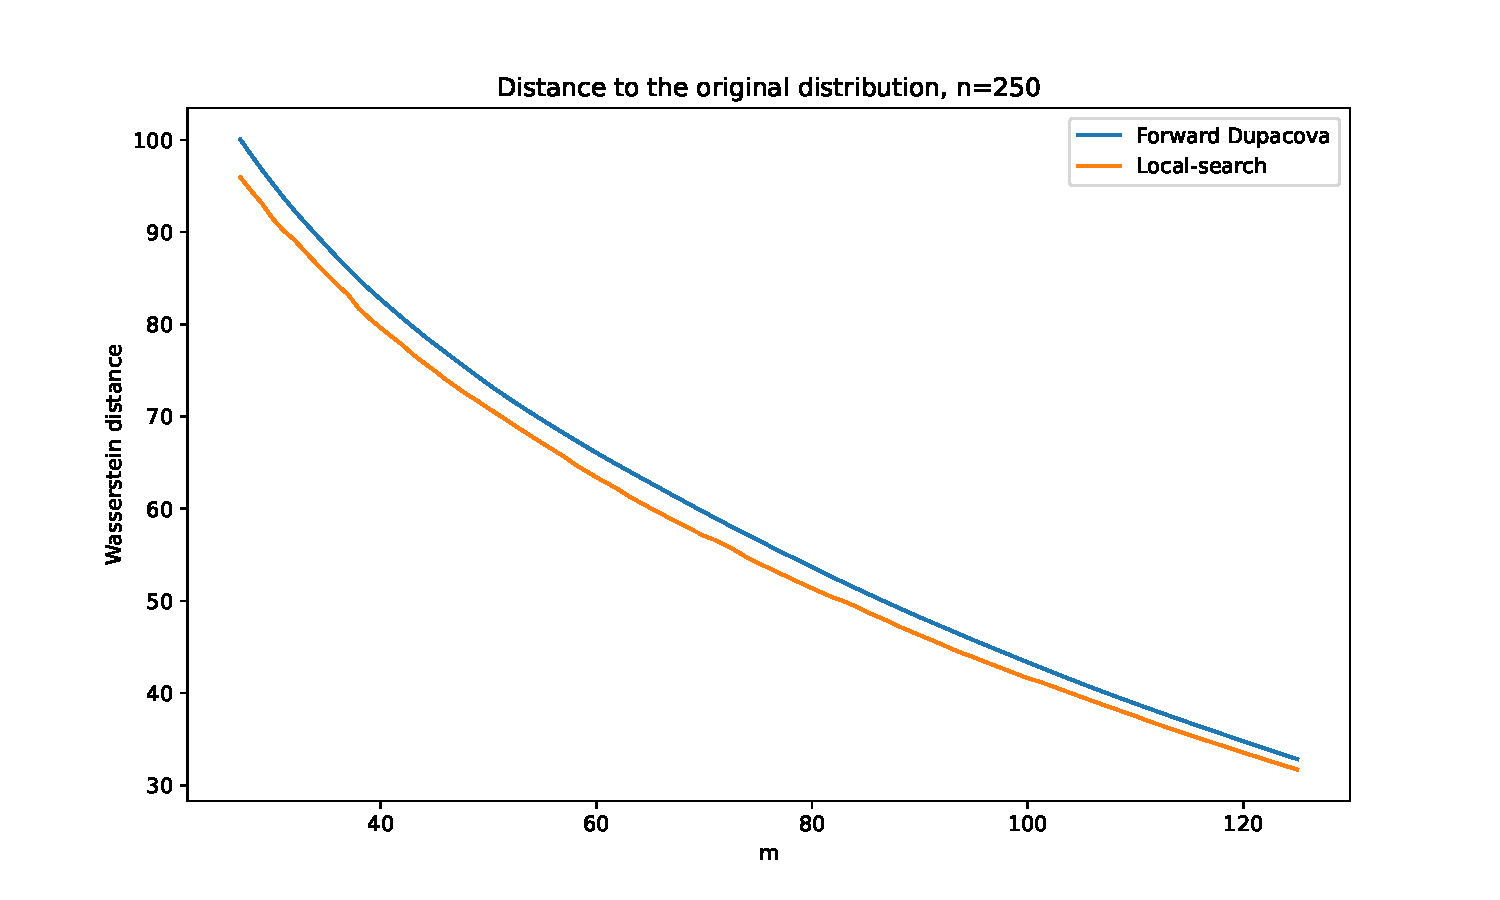
\includegraphics[width=0.47\textwidth]{plots/distance two stage.pdf} 
    }
    \hfill
    \subfloat[Ratio]{
        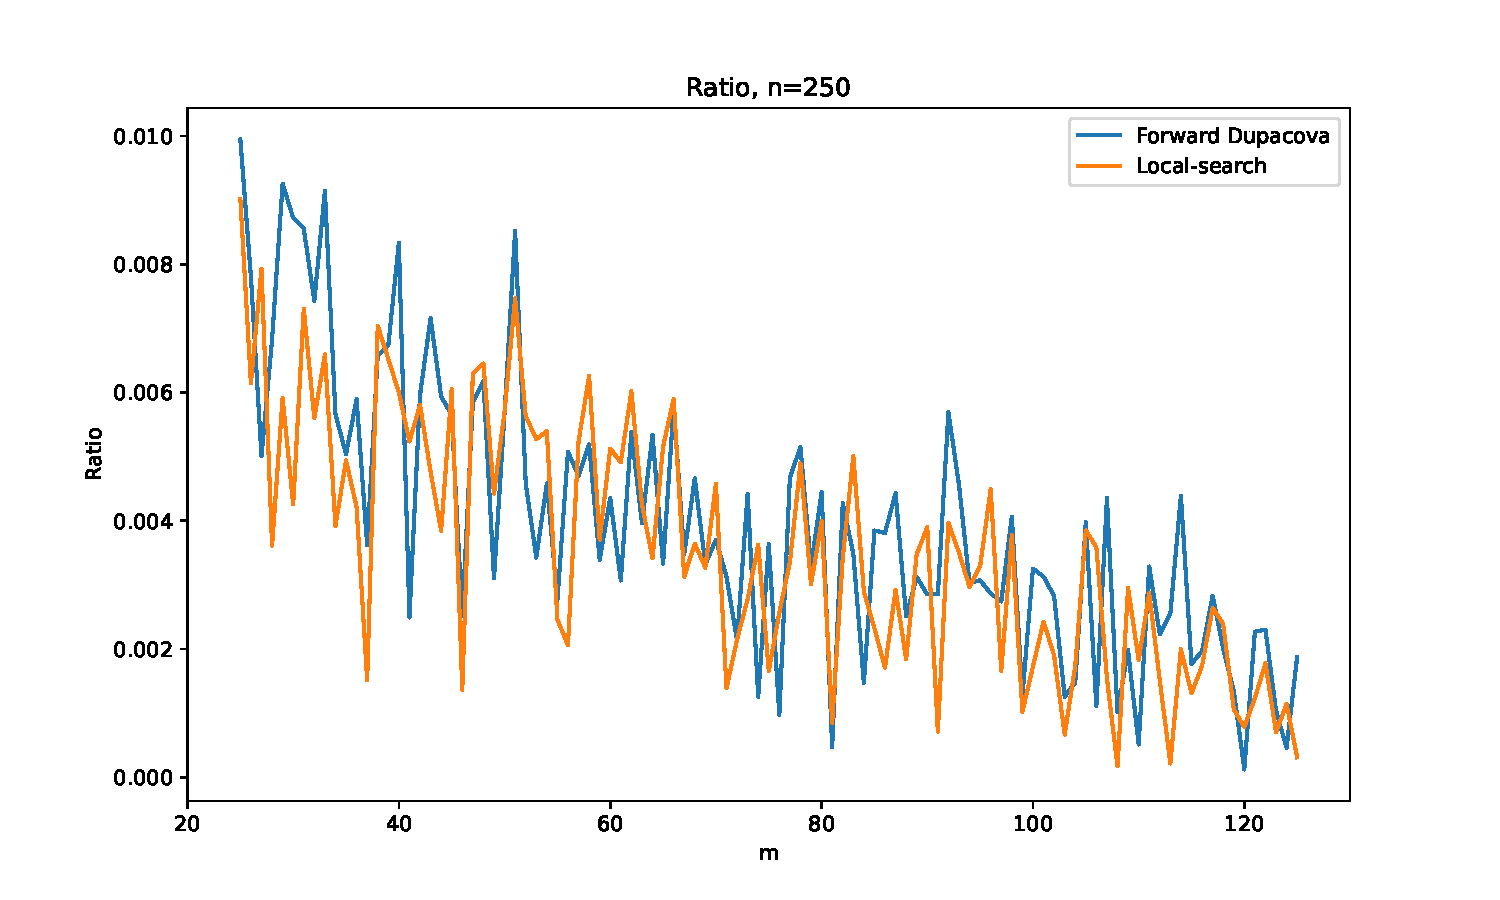
\includegraphics[width=0.47\textwidth]{plots/ratio 250 two stage.pdf} 
    }
    \hfill
    \subfloat[Run time]{
        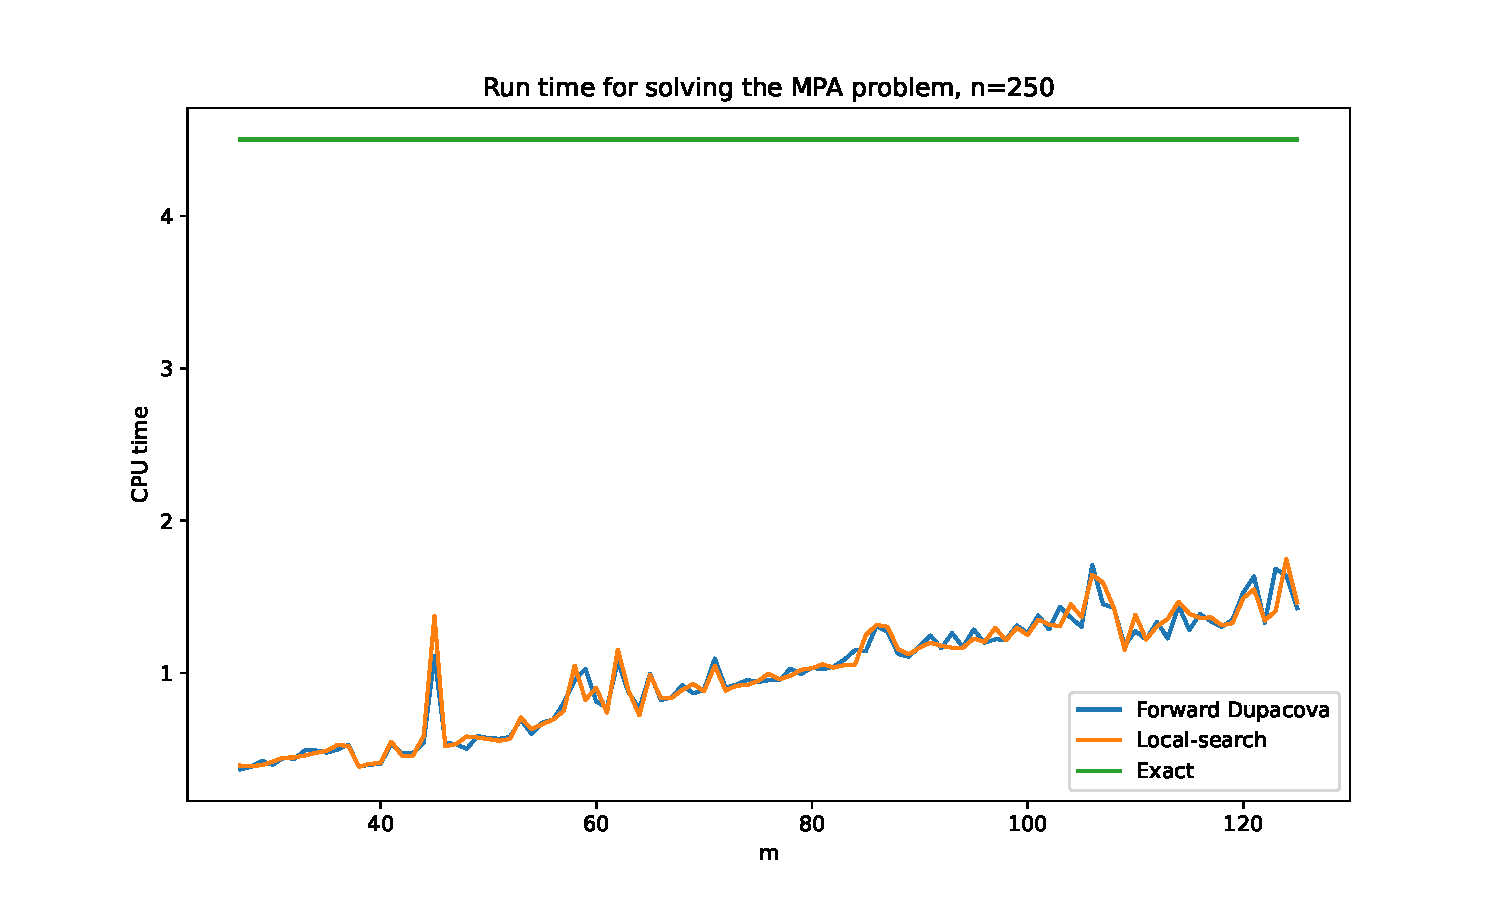
\includegraphics[width=0.47\textwidth]{plots/run time two stage.pdf} 
    }
    \caption{Figures for two-stage stochastic programming with $n=250$.}
\end{figure}

These figures present: Wasserstein distance between the original distribution and reduced ones (either via local-search or greedy algorithm), the optimal value ratio and run time. Both local-search and greedy algorithm give comparable ratios (less than 2\% when reducing the number of scenarios by a factor 10) even though local-search tends to give better approximation as it gives a distribution that is generally closer to the original one. Obviously when $m$ grows, distribution generated are closer to the original one, hence, it gives a smaller ratio in general. This observation is comforting with the Lipschitz nature of the problem: $$\lvert v\left(P\right)-v\left(Q\right)\rvert \leq C d_\ell\left(P,Q\right)^\ell.$$ A distribution that is closer to the original one will generally lead to a closer optimal value. There can be a gap sometimes. Run time grows linearly with $m$ because Gurobi is very efficient for small scales LP. Solving the LP \ref{LP} with $n=2000$ takes about 29 seconds, when the reduced LP with $m=200$ is completed in about 2 seconds. Cutting the number of scenarios by a factor 10 is clearly not threatening here and reduces run time. Generating this new scenario set can be excruciating but still it can be very interesting in some cases e.g. if you dare optimizing on cost vector in a multiproduct assembly problem with a certain distribution of demands. You can reduce once demands and then use the reduced distribution to save run time when solving again and again the LP.
\section{Conclusion}
\clearpage
\bibliography{biblio}
\bibliographystyle{alpha}
\clearpage
\appendix

\section*{Appendix A}
\addcontentsline{toc}{section}{Appendix A}

\section*{Appendix B}
\addcontentsline{toc}{section}{Appendix B}

\end{document}
